\svnidlong
{$LastChangedBy$}
{$LastChangedRevision$}
{$LastChangedDate$}
{$HeadURL$}

\chapter{Local structure identification in real space}
\label{ch:structure_id}
%Author: \svnauthor; Revision: \svnrev; Last changed on: \svndate; URL: \url{\svnkw{HeadURL}}
% Create a new 1st level heading
\section{Introduction}
\subsection{Crystallography}

From the end of the 18th century, natural scientists rediscovered the atoms invented by the ancients. In parallel, they began to explore the structure of condensed matter, starting by crystals. Rene-Just Hauy~\citep{Hauy1784} imagined that the peculiar proportions and angles of crystals were due to the shape of their elementary building bricks. Gabriel Delafosse~\citep{Delafosse1840} made the essential distinction between an atom and this crystal brick: the brick is an elementary structure made of atoms (or molecules). Auguste Bravais~\citep{Bravais1866} made the inventory of the 14 possible crystal lattices, corresponding to the 32 point symmetry groups.

The idea that crystals are periodically ordered was amazingly successful. Crystallographers were able to predict all the characteristic angles that could appear between the facets of crystals of any given type. With the discovery of x-ray diffraction (see \SectionRef{Diffraction}) in crystals by Max von Laue~\citep{Laue1912} in 1912 and the subsequent development of x-ray crystallography by William H. and William L. Bragg~\citep{bragg1965crystalline} the theory of crystallography received an unequivocal stamp of approval.

\begin{figure}
	\centering
	\subfloat[\acs{FCC}]{\label{fig:FCC}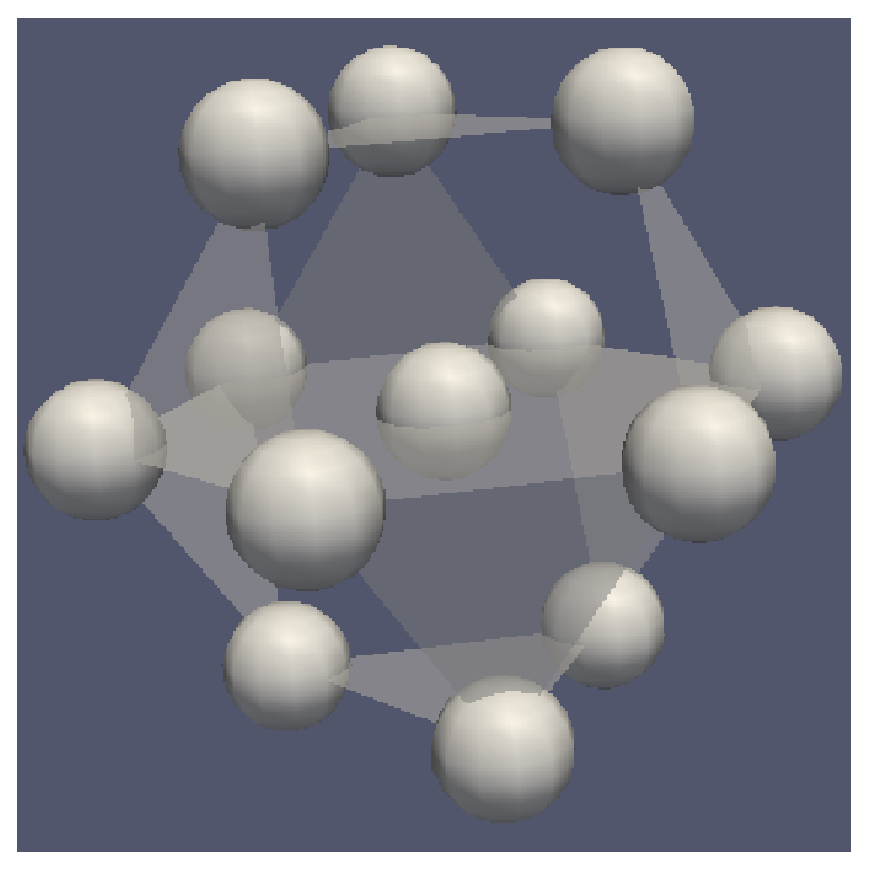
\includegraphics[width=0.3\textwidth]{fcc_13}}
	\subfloat[\acs{HCP}]{\label{fig:HCP}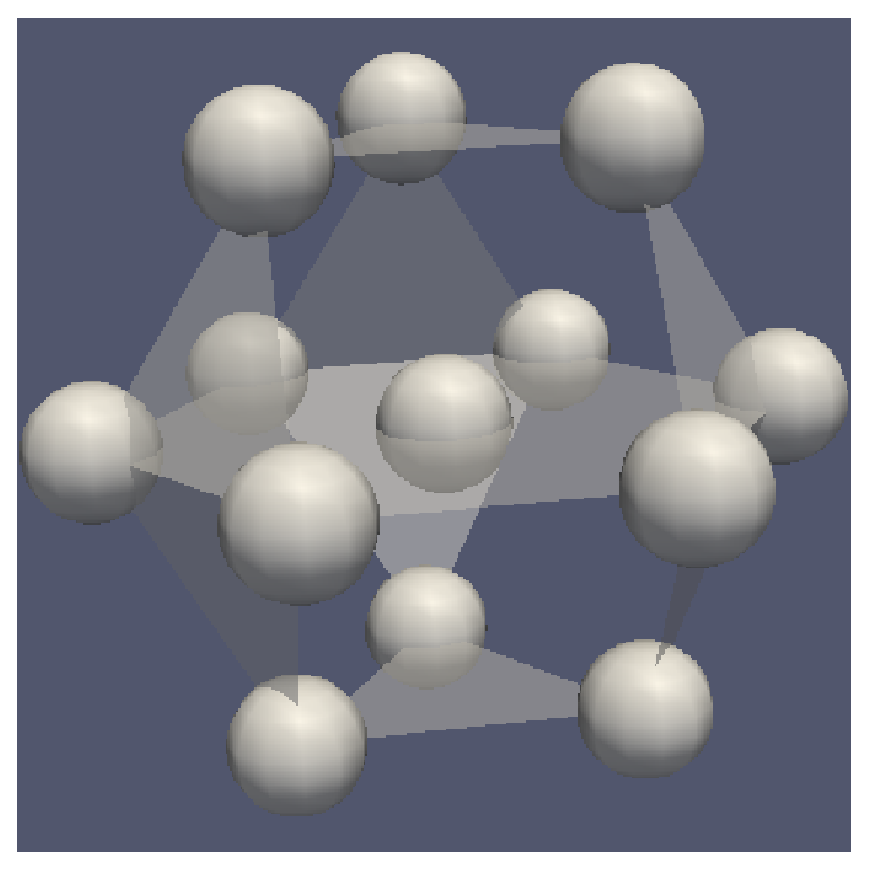
\includegraphics[width=0.3\textwidth]{hcp_13}}
	\subfloat[Icosahedron]{\label{fig:ico}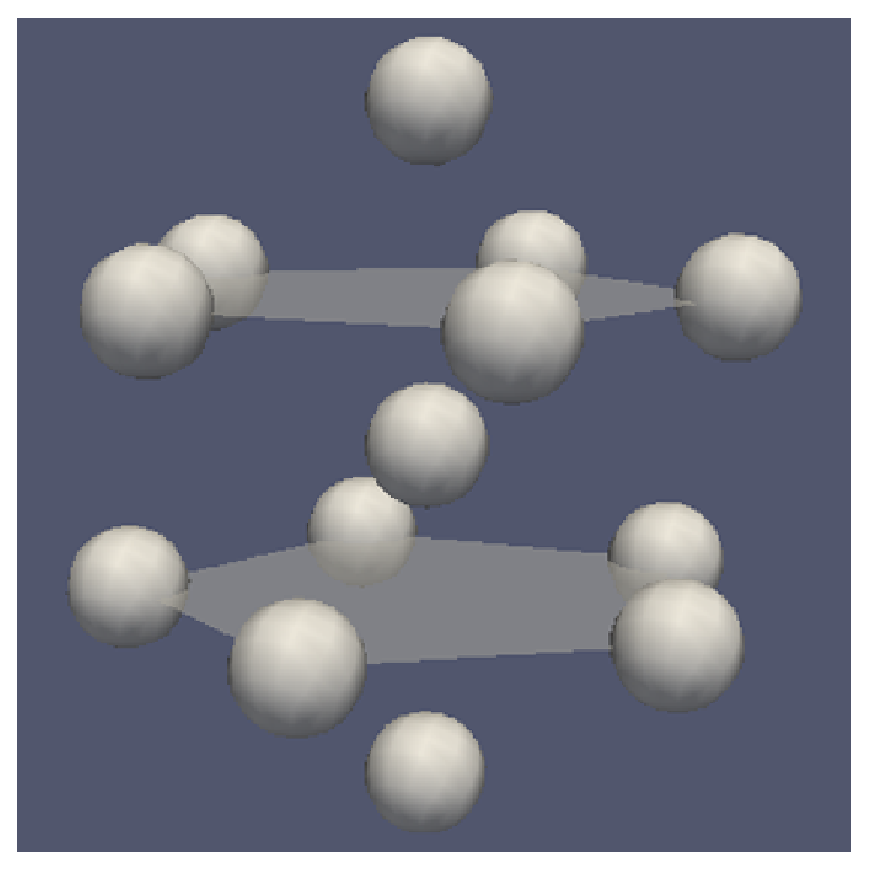
\includegraphics[width=0.3\textwidth]{ico_13}}
	\caption{The three possible clusters made of 12 spheres in contact with a central sphere.}
	\label{fig:basicClusters}
\end{figure}

\begin{figure}
	\ContinuedFloat
	\centering
	\subfloat[9 particles \acs{BCC}]{\label{fig:BCC9}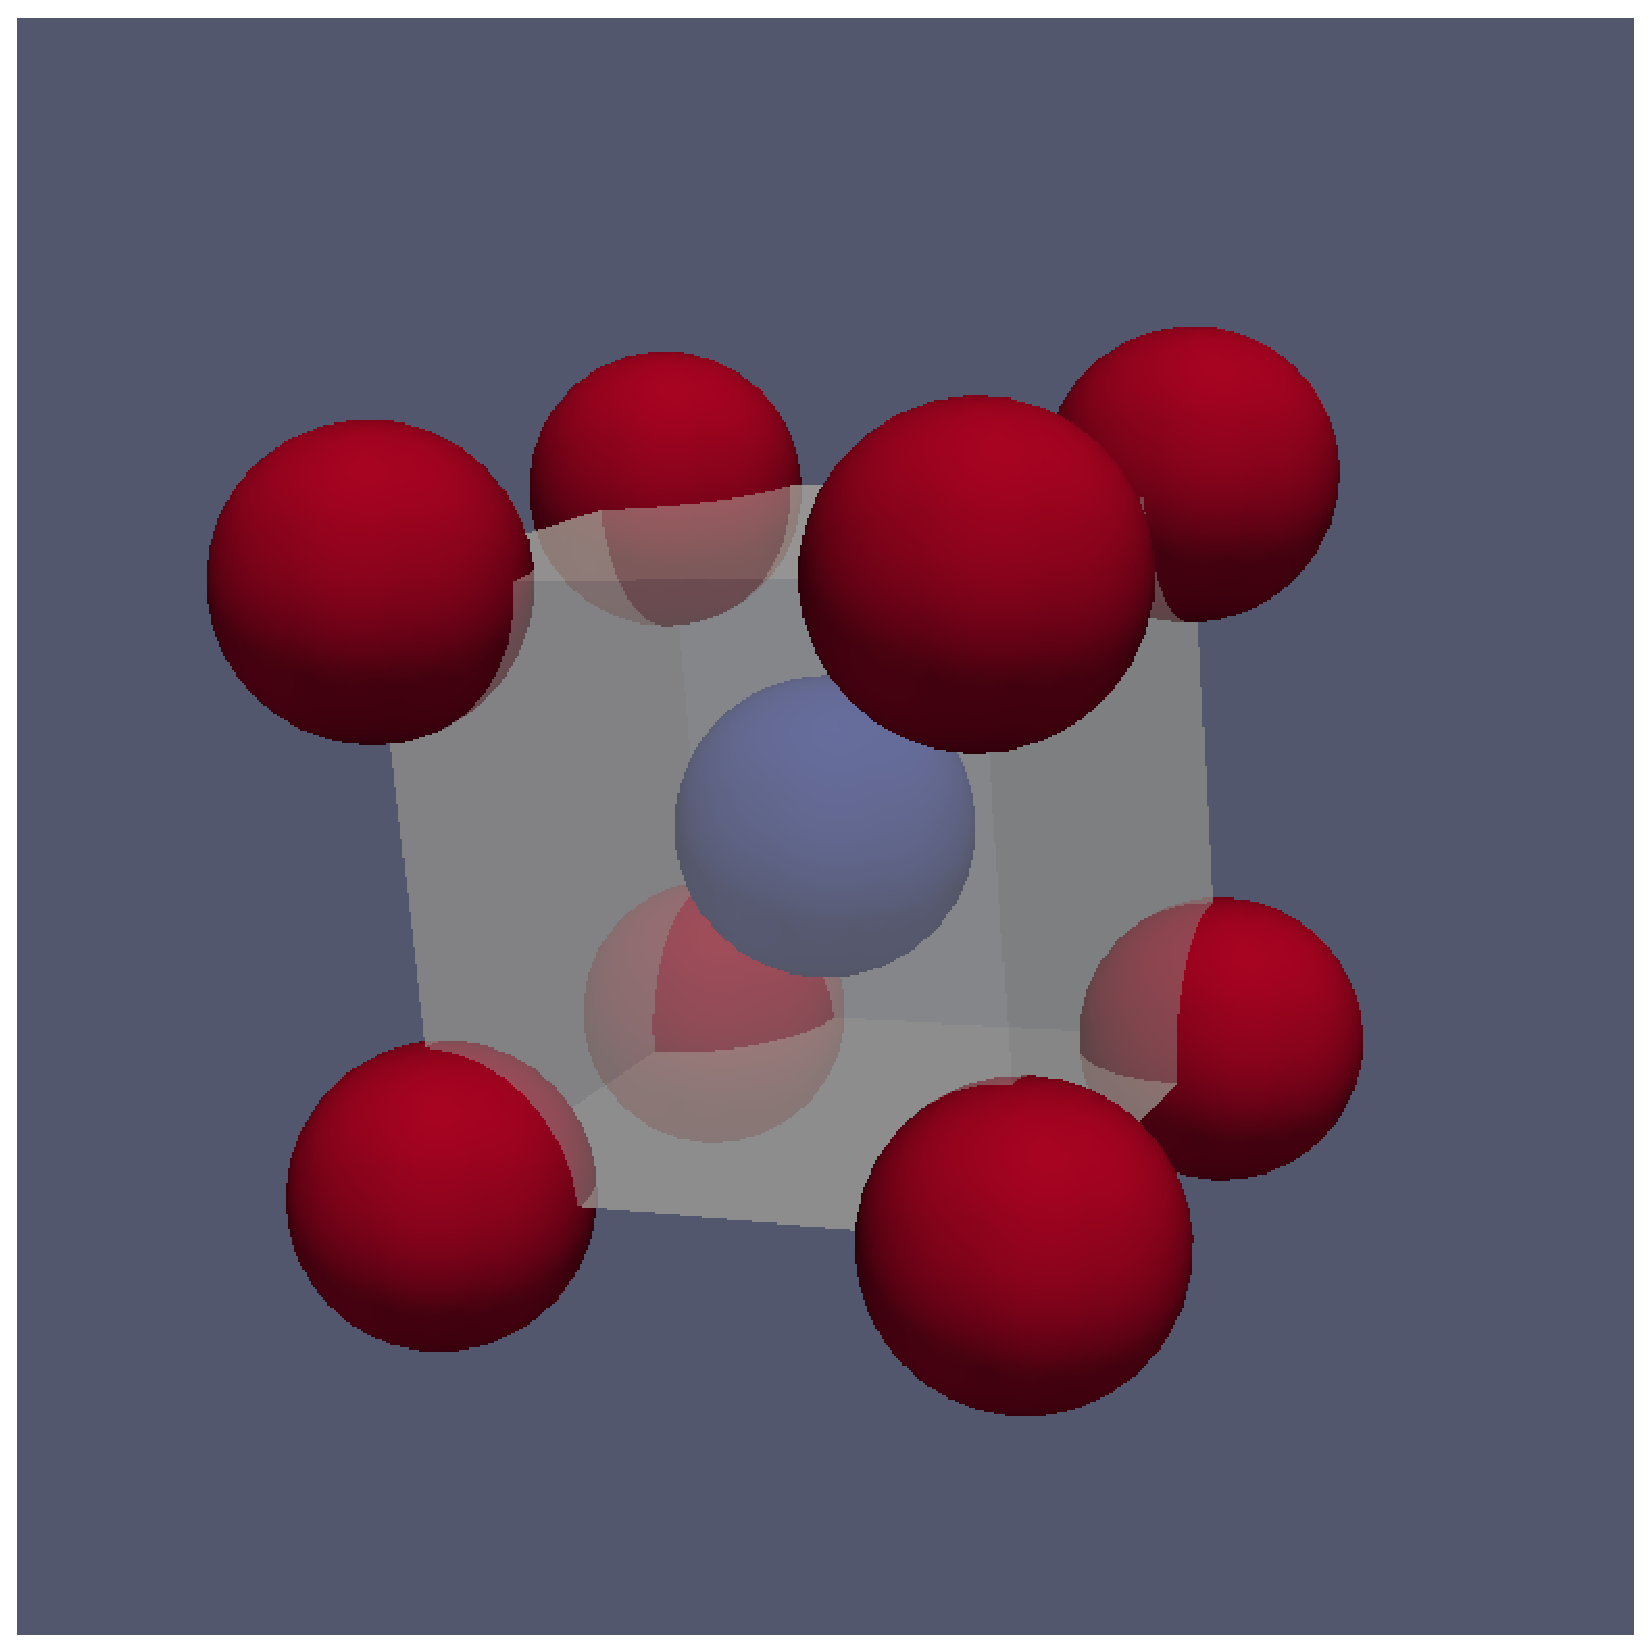
\includegraphics[width=0.3\textwidth]{bcc_9}}
	\subfloat[15 particles \acs{BCC}]{\label{fig:BCC15}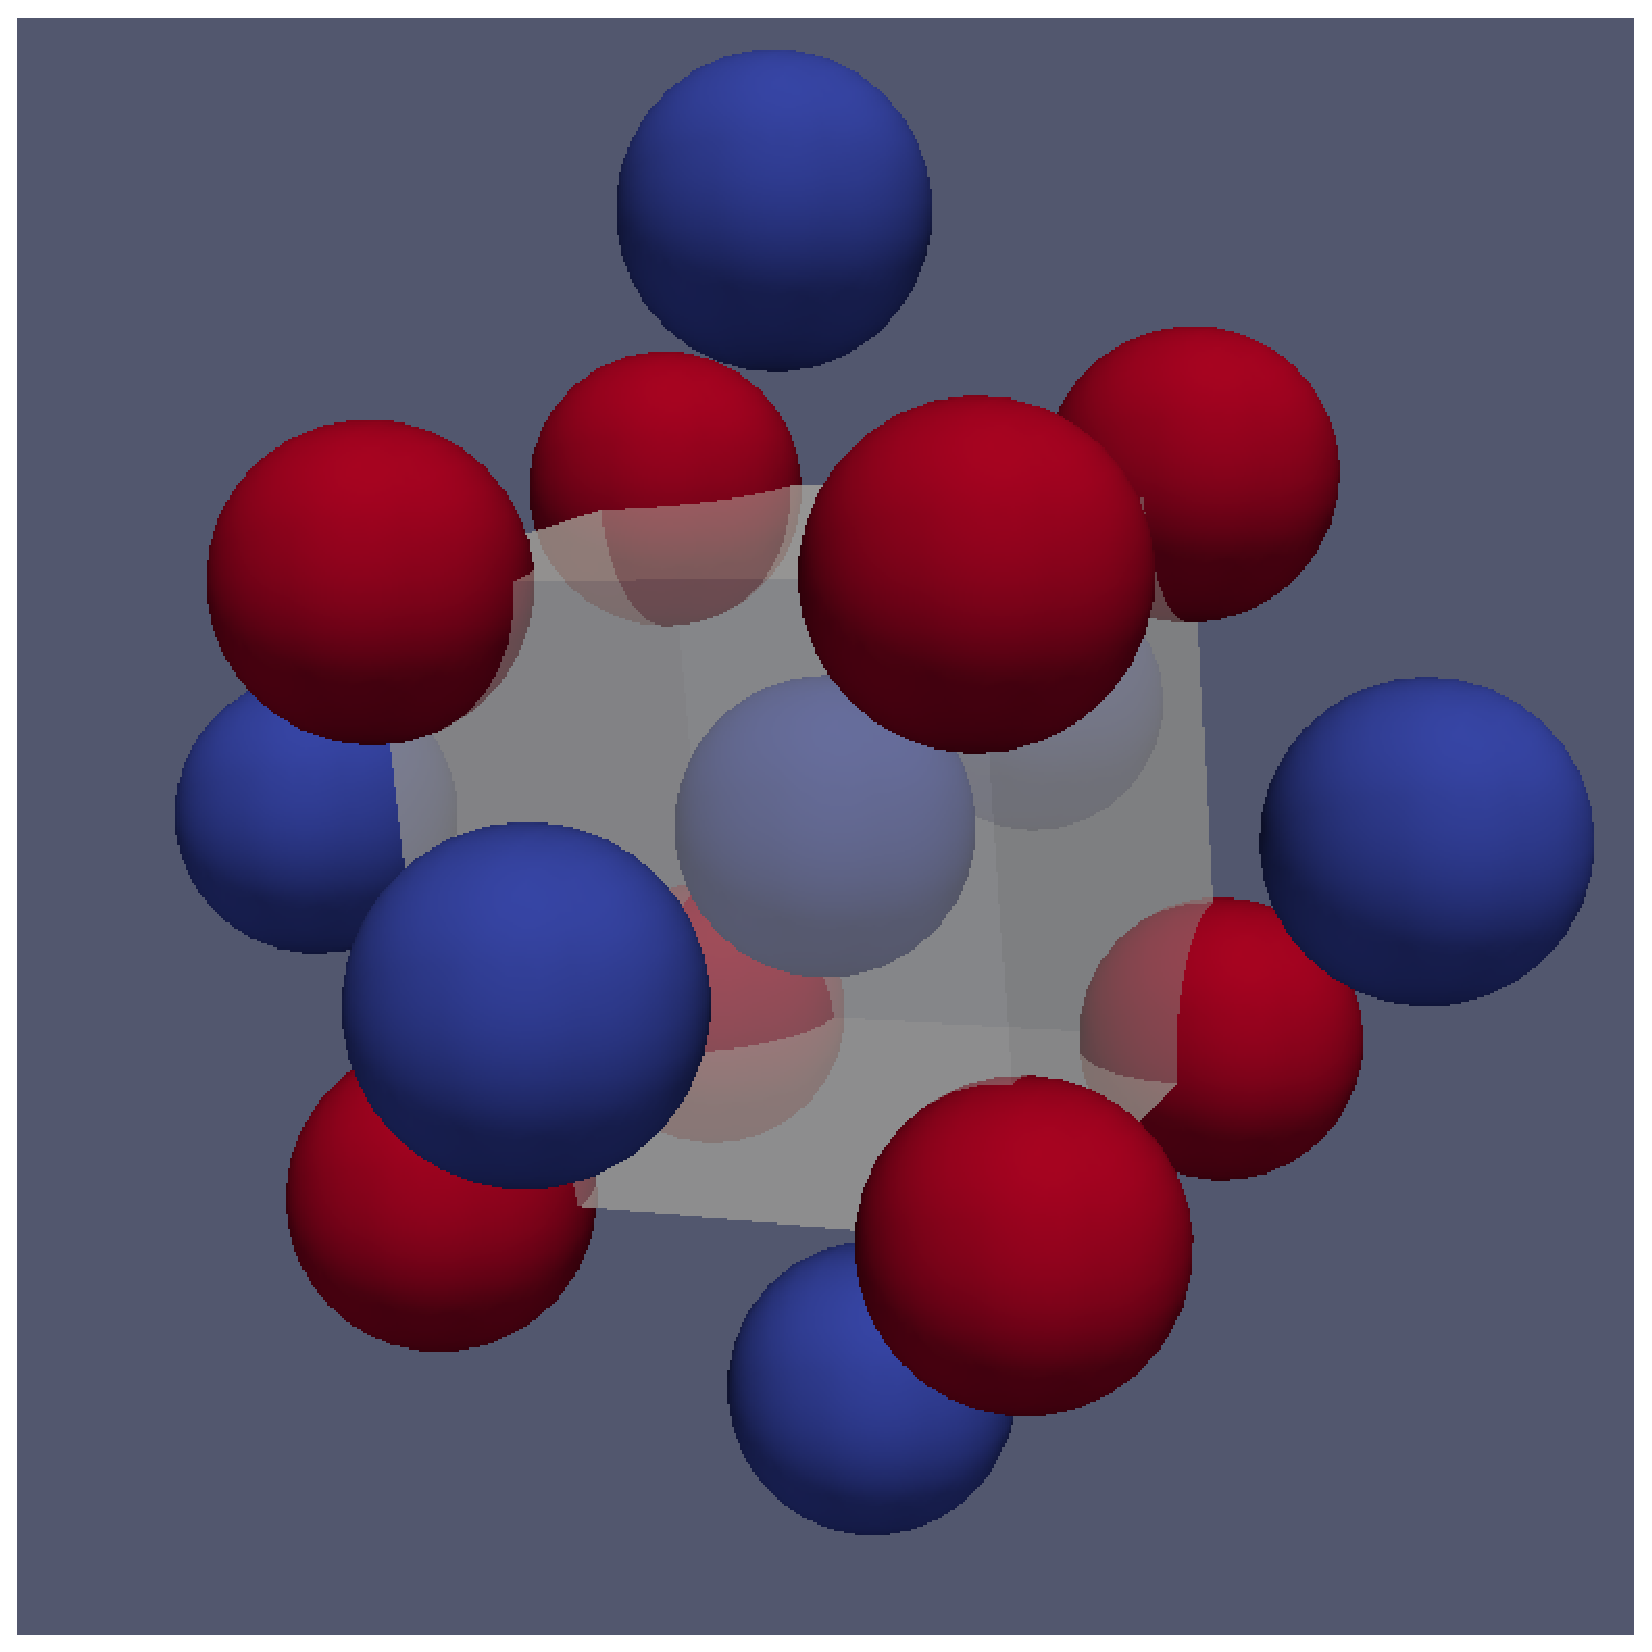
\includegraphics[width=0.3\textwidth]{bcc_15}}
	\subfloat[Dodecahedron]{\label{fig:dodecahedron}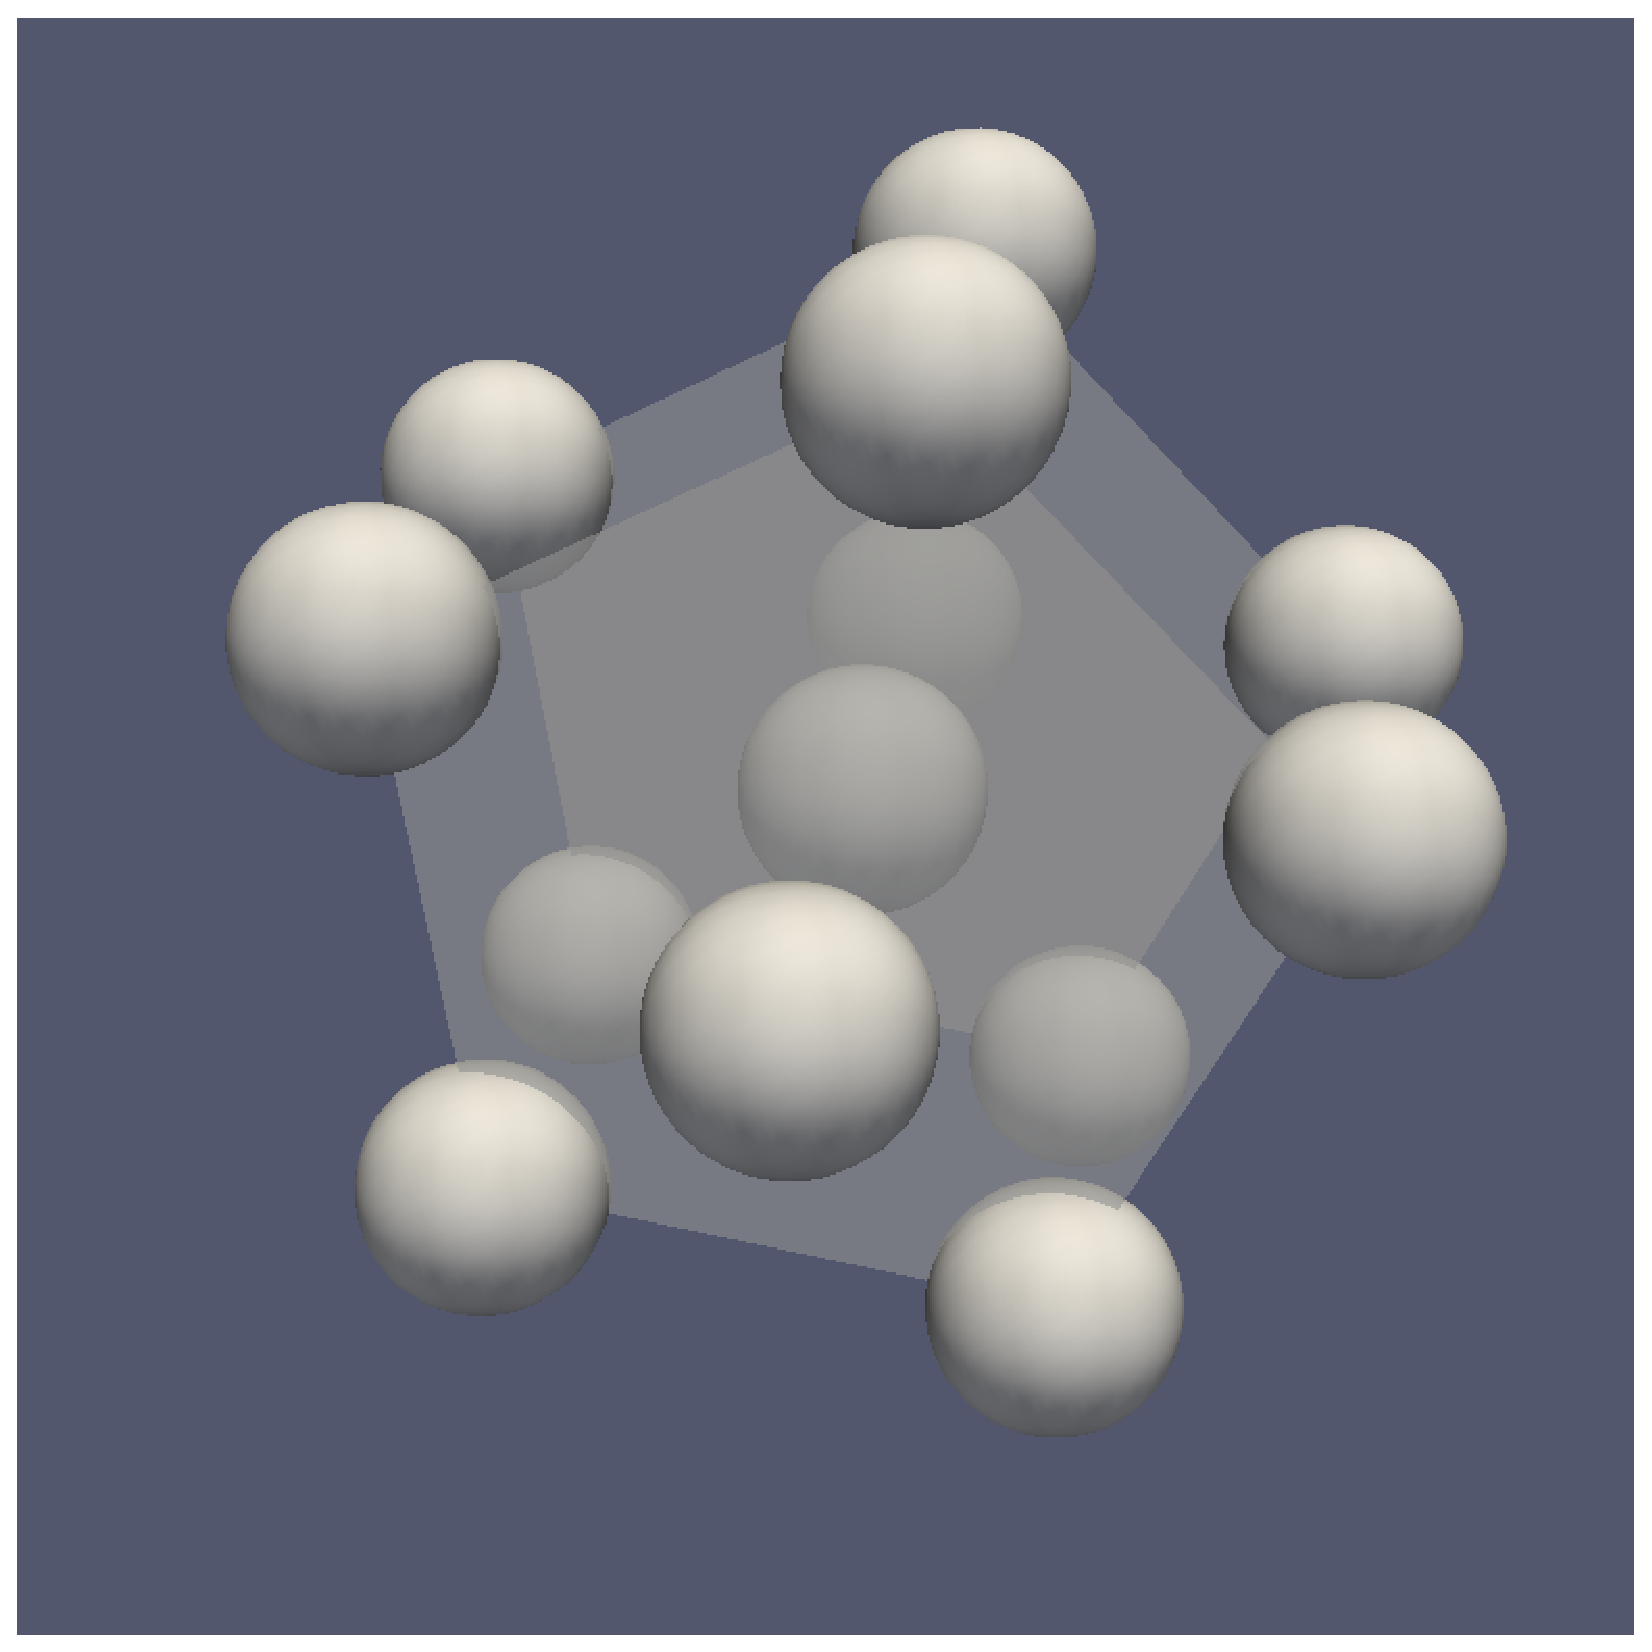
\includegraphics[width=0.3\textwidth]{dodec_13}}
	\caption{Other simple clusters.}
	\label{fig:other_clusters}
\end{figure}

\subsection{Non-crystalline condensed matter}

Disordered structures are not random structures. There is still order in an amorphous or a liquid material. The main point is the lack of periodicity which was the reference for the definition of the order. Periodic crystalline order supposes three types of order: local order, positional order and orientational order. Quasi-crystals, discovered in the 1980's~\citep{Shechtman1984} have a clear orientational order (\FigureRef{fig:diffraction}) but without any periodicity (positional order). In amorphous or liquid structures only the local order remains.

In the metallic structure with isotropic interaction, the local order is similar to the one obtained in a packing of soft balls. All particles have roughly 12 neighbours. But has observed by Frank~\citep{Frank1952}, the 13 particles icosahedral arrangement (see \FigureRef{fig:ico}), incompatible with space tiling, has a significantly lower energy than the \ac{FCC} (\FigureRef{fig:FCC}) and \ac{HCP} (\FigureRef{fig:HCP}) arrangement, at least for the simple Lennard-Jones pair potential. This is a very simple example of local order. In covalent structures like silicon there are oriented interactions leading to the tetracoordinated local order which is a more complex example, but in all cases a local order can be defined. So, a dense phase cannot be completely disordered like a gas, and this has very important consequences for mechanical and physical properties (heat conduction, phase transition, etc.).

\subsection{Diffraction}
\label{Diffraction}

\begin{figure}
	\centering
	\subfloat[Schematic principle of X-ray diffraction.]{\label{fig:diffraction_sketch}\def\svgwidth{0.5\textwidth}\input{xray.pdf_tex}}
	\subfloat[Typical diffraction diagram of a quasicrystal.]{\label{fig:quasiX}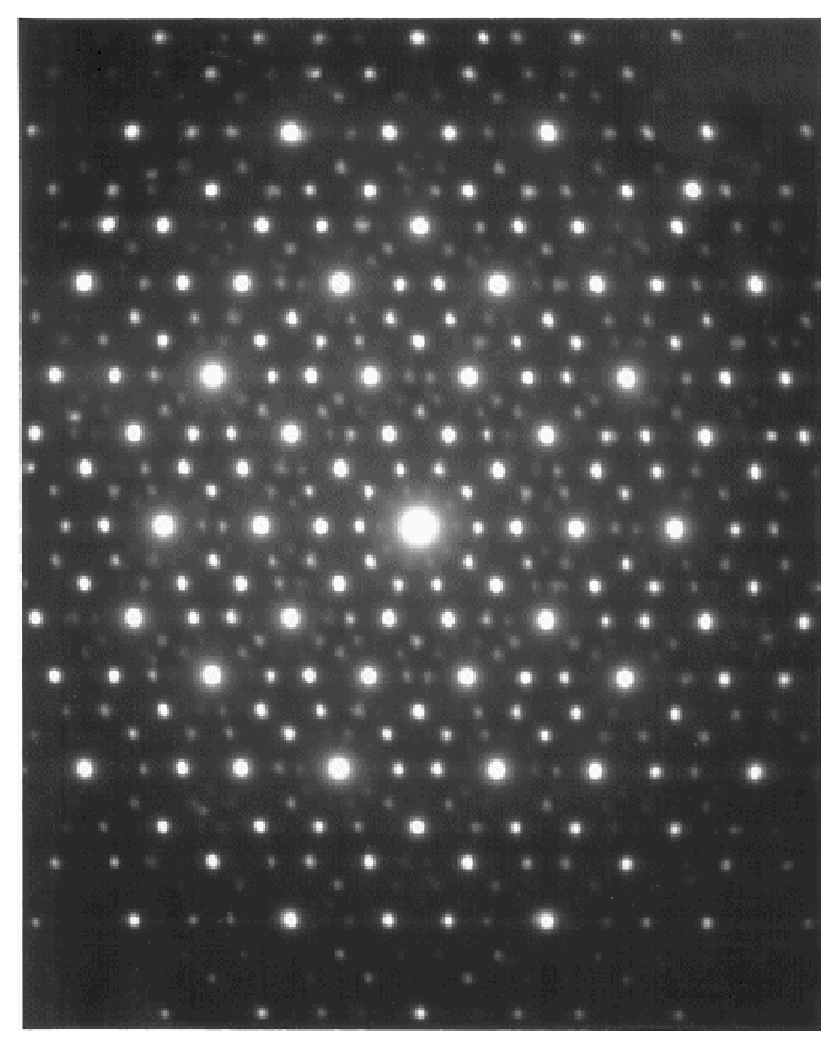
\includegraphics[width=0.4\textwidth]{diffraction_quasiX}}
	\caption{The diffraction patterns indicate \subref{fig:diffraction_sketch}~6-fold and \subref{fig:quasiX}~5-fold or 10-fold rotational symmetry.}
	\label{fig:diffraction}
\end{figure}

Since 1912 and the experiments of Max von Laue~\citep{Laue1912}, the structure of condensed matter can be explored by diffraction. A beam of X-rays, neutron or electrons has a sufficiently short wavelength to probe the material at the atomic scale. The diffracted beam cannot be focused to produce images, so the sample structure must be reconstructed from the diffraction pattern. Sharp features in the diffraction pattern arise from periodic, repeating structure in the sample, which are often very strong due to coherent reflection of many photons from many regularly spaced instances of similar structure, while non-periodic components of the structure result in diffuse (and usually weak) diffraction features.

Conventional diffraction techniques only allow to extract structural information averaged over the illuminated sample area. If a structure is smaller than this area, its signature is averaged out by the surrounding incoherent structures~\citep{Wochner2009}.

Because of their highly ordered and repetitive structure, crystals give diffraction patterns of sharp Bragg reflection spots (\FigureRef{fig:diffraction}). However, amorphous or soft materials are much more difficult to analyse. Non-periodic local structures - sometime important for the physics and the mechanical properties of the material - are often hidden by the configurational averaging.

\subsection{Granular matter, colloids and simulation}

A way to study medium range or local structures by diffraction is to use larger particles, scaling up everything except the illuminated area. So that local structures size become comparable to the illuminated area.

For example, one can use colloids, \latin{i.e.} \unit{100}{\nano\meter} to a few microns objects subject to Brownian motion and thus exploring space like atoms. Colloids can behave as hard spheres or can be given interaction potentials: purely repulsive due to charges, or attractive due to the depletion interaction. They are able to form various state of matter like gas, liquids, crystals, gels and glass. Colloids are model atoms.

With the larger colloids, larger than the wavelength of visible light, direct optical imaging is possible. Using confocal microscopy, it is even possible to track the coordinates of tens of thousand particles in three dimensions (see \ChapterRef{ch:tracking}). The accessible data is then real space data, not diffraction spectrum in Fourier space.

Another possible model atom system is granular matter: sand, steel balls or rice seeds, etc. When granular matter is fed energy (shaking, periodic shear, etc.), the particles explore space almost like atoms. They can constitute fluids, solids (amorphous or crystal). Gains also can be tracked in real space (often 2D).

Finally, computer simulations (molecular dynamics, \acl{BD}, etc.) yield natively their results in real space.

\subsection{Why structure identification in real space?}

We have enumerated a few systems yielding naturally real space sets of coordinates rather than reciprocal space data. Because diffraction is still the reference probe of condensed matter, it was natural at first to translate the real space coordinates into the scattering function in order to identify structures. But at the end of the day, we are looking for real space structures. Some ways must exist to identify structure directly in real space.

Moreover, most of the scattering techniques yield informations about the positional order of particles. The characteristic angles of the structure is deducted only at a macroscopic, at best mesoscopic, scale. Real space techniques should yield locally such information.

\section{Neighbours and bonds}
\label{sec:neighbours_bonds}

To identify a structure, we have to know which particles are related to each other. In the absence of long range interactions - this is the case when we are looking for local structures - it means finding the neighbours of each particle, or the bond network.

% Create a new 2nd level heading
\subsection{Bonds due to an attractive potential}

The notion of neighbour is simple in the case of an attractive potential presenting a well deeper than a few $k_{B}T$, like the well known Lennard-Jones (LJ) potential or the Asakura-Oosawa (AO) potential. At a given (low enough) temperature, the potential has a certain range $r_b$ and the particles closer than this range are defined as bonded.

\subsection{The \texorpdfstring{\acf{RDF}}{\acl{RDF}}}
\label{sec:rdf}

\begin{figure}
	\centering
	\subfloat
		[Radial distribution function of colloidal hard sphere glass. Note that the first shell and the second shell are separated by a clear minimum: the maximum bond length.]
		{\def\svgwidth{0.5\textwidth}\input{typicalRdf.pdf_tex}}
	\subfloat
		[$g(r)$ from hard sphere simulations of a liquid at the freezing point (solid line) and of a crystal at the melting point(dashed line). Source \ReferenceRef{Truskett1998}.]
		{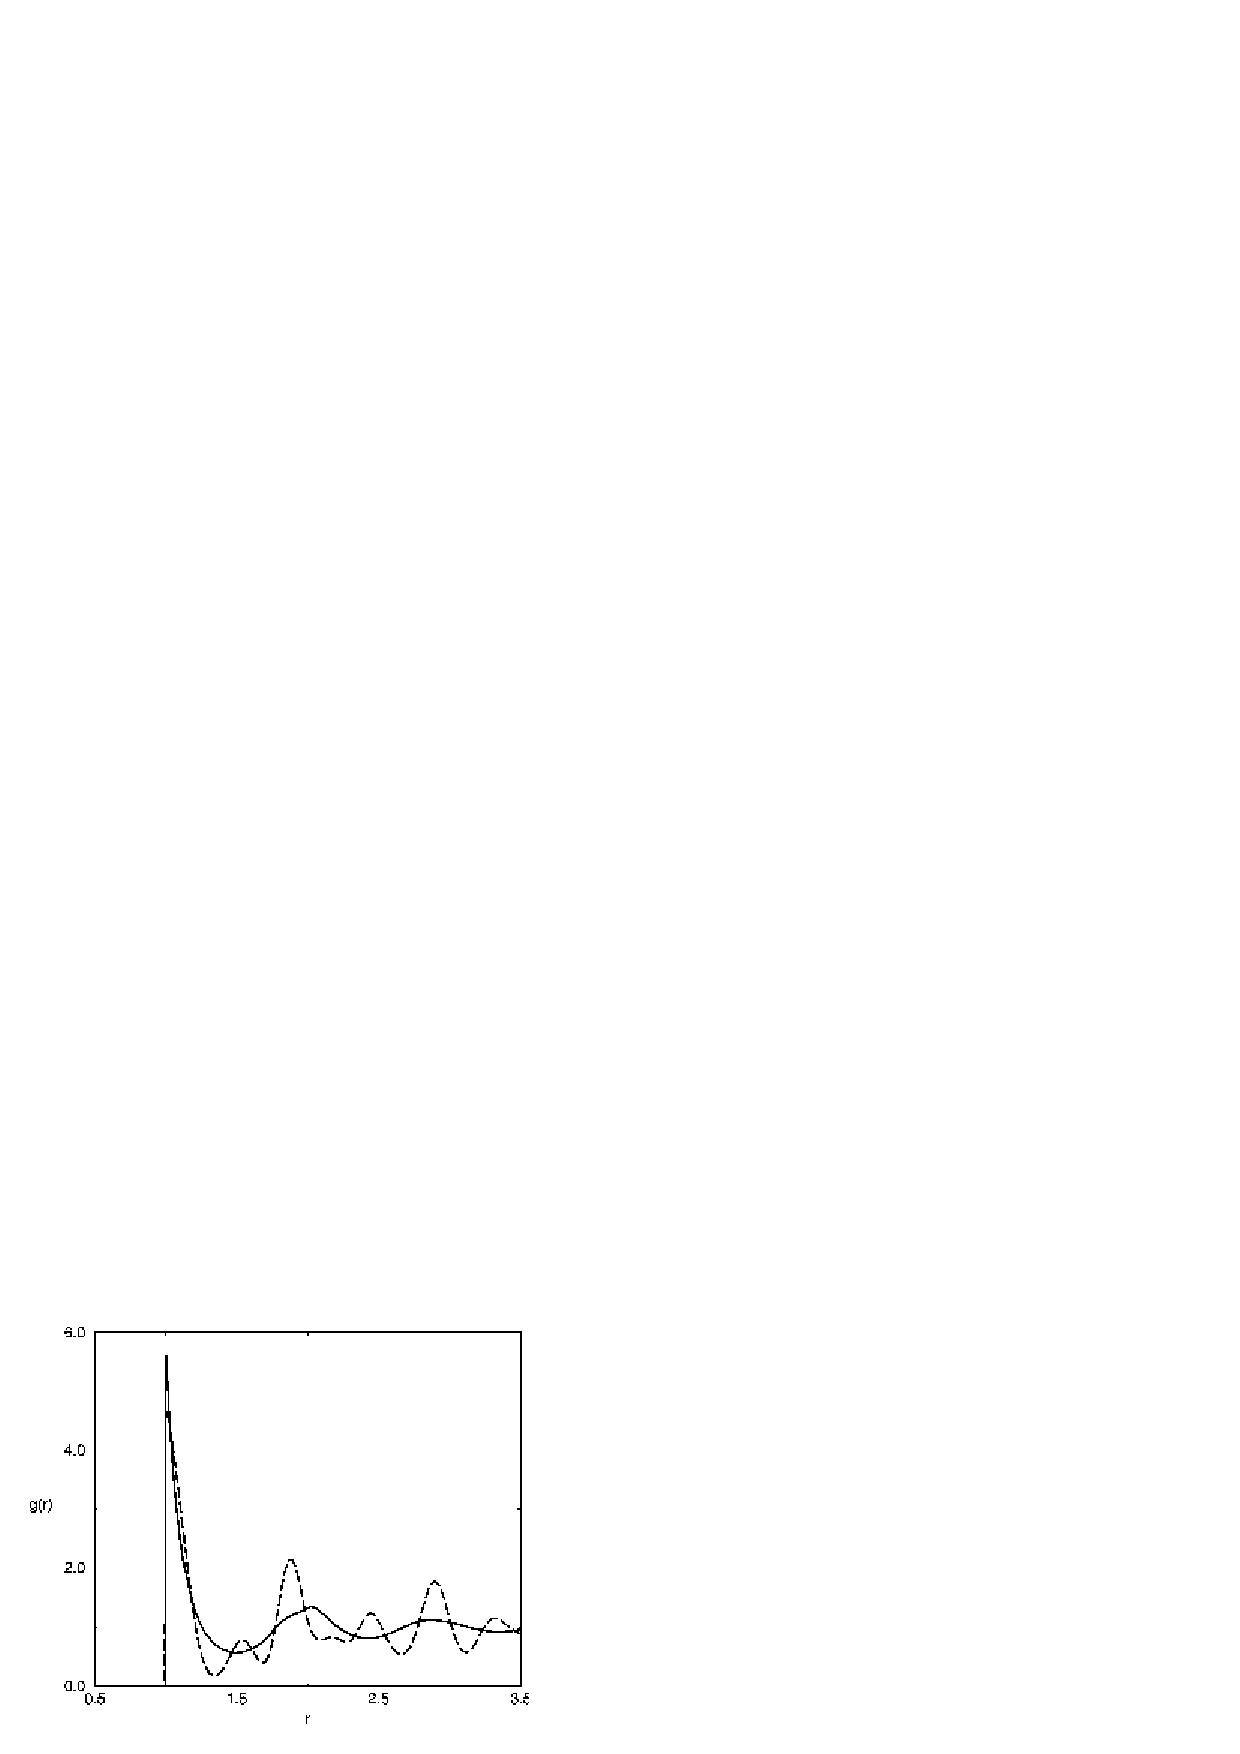
\includegraphics[width=0.4\textwidth]{rdf_XF}}
	\caption{Examples of \acf{RDF}.}
	\label{fig:rdf}
\end{figure}

The \acf{RDF} describes how the particle density varies as a function of the distance from one particular particle. It is defined as the ratio of the probability to find a particle at a distance $r$ of the central particle by the same quantity in the ideal gas:
\begin{equation}
	g(r) \equiv \frac{1}{N} \sum_{i}^N \frac{
		\sum_{j\neq i} \delta(r_{ij} - r)
		}{
		\int_V \rho \delta(r^\prime-r) dV
		}
	\label{eq:rdf}
\end{equation}
where $\rho$ is the number density. In the bulk, the numerator has a a simple expression independent of the central particle and $g(r)$ is written as:
\begin{equation}
	g(r) = \frac{
		\sum_{i}^N \sum_{j\neq i} \delta(r_{ij} - r)
		}{
		4\pi r^2 dr \rho(N-1)
		}
	\label{eq:rdf_bulk}
\end{equation}

By definition, in an ideal gas we have $g(r)=1$ for all distance $r$. For an dilute hard spheres gas, the \ac{RDF} is a step function: no particle within the hard core and uniform probability further. In a crystal, the \ac{RDF} presents thin peaks indicating a regular periodic arrangement. In a dense phase, the \ac{RDF} presents oscillations, or broad peaks that indicates preferred distances (see \FigureRef{fig:rdf}). The first peak is the first shell of particles around the reference particle; the second peak the second shell, etc.

When the \ac{RDF} presents a clear fist minimum as in \FigureRef{fig:rdf}, it is possible to use its position to define the maximum bond length $r_b$. Purely repulsive potentials (hard sphere, \ac{WCA}, etc.) satisfy this condition in dense phases.

In practice, the \ac{RDF} is an averaged function that does not contain information about local non-periodic structures. The \ac{RDF} is a real space function, but it is directly related to the static \ac{Sq} given by scattering experiments.
\begin{equation}
	S(q) = 1 + \rho \int {\exp{(-\imath \vec{q}\cdot\vec{r})} g(r)dr}
	\label{eq:rdf2Sq}
\end{equation}



\subsection{Voronoi diagram}

\begin{figure}
	\centering
	\subfloat[2D. Source Wikipedia]{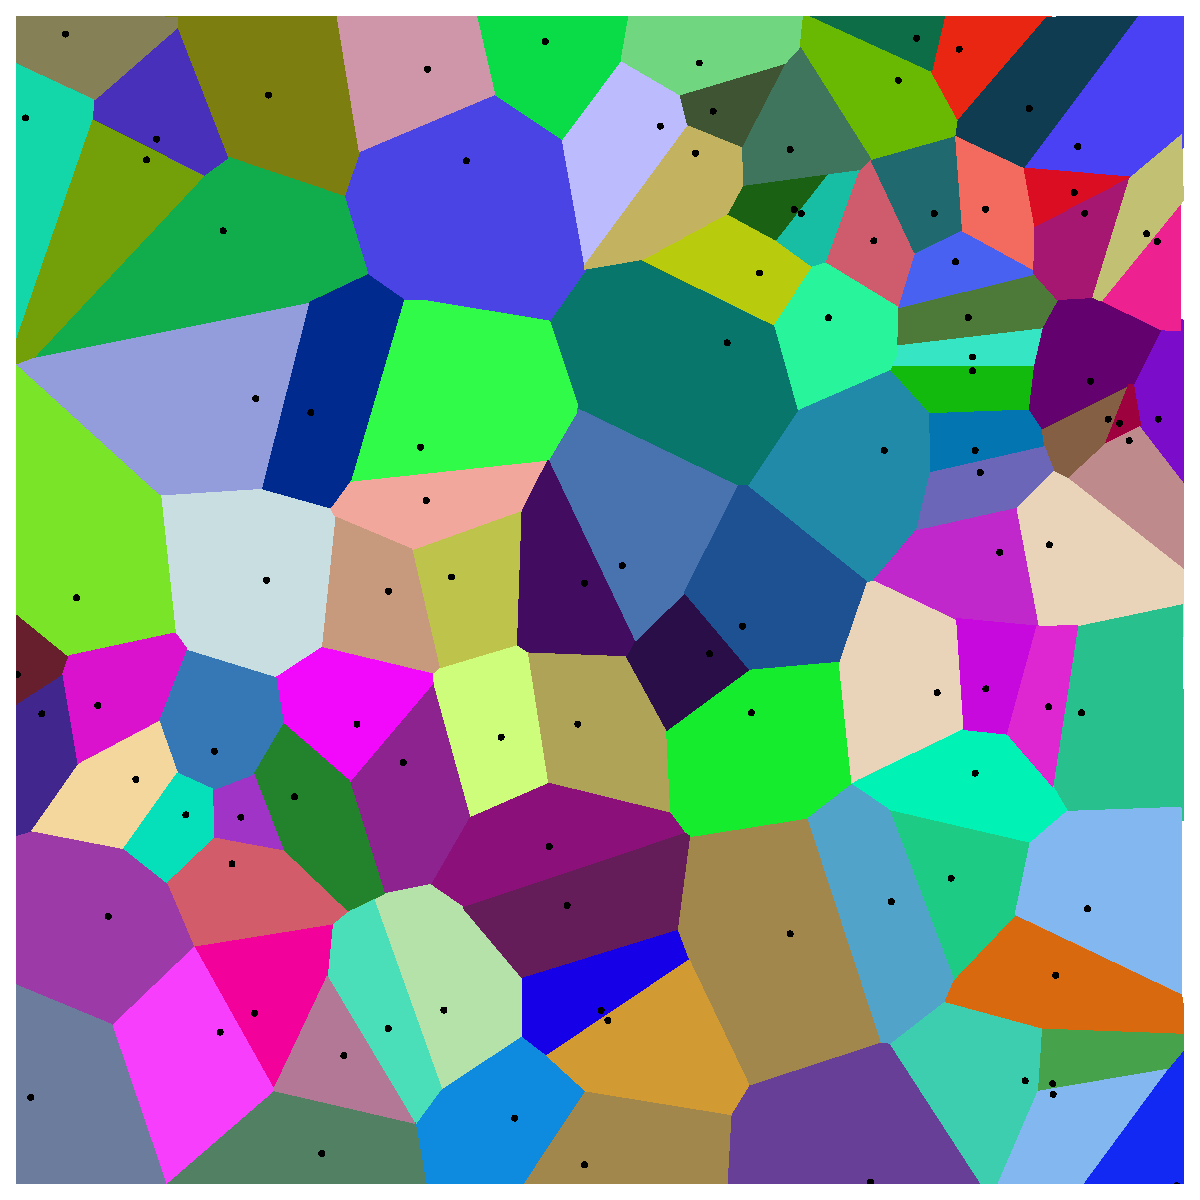
\includegraphics[width=0.45\textwidth]{voro2d}}
	\subfloat[3D. Source~\citep{rycroft2007multiscale}]{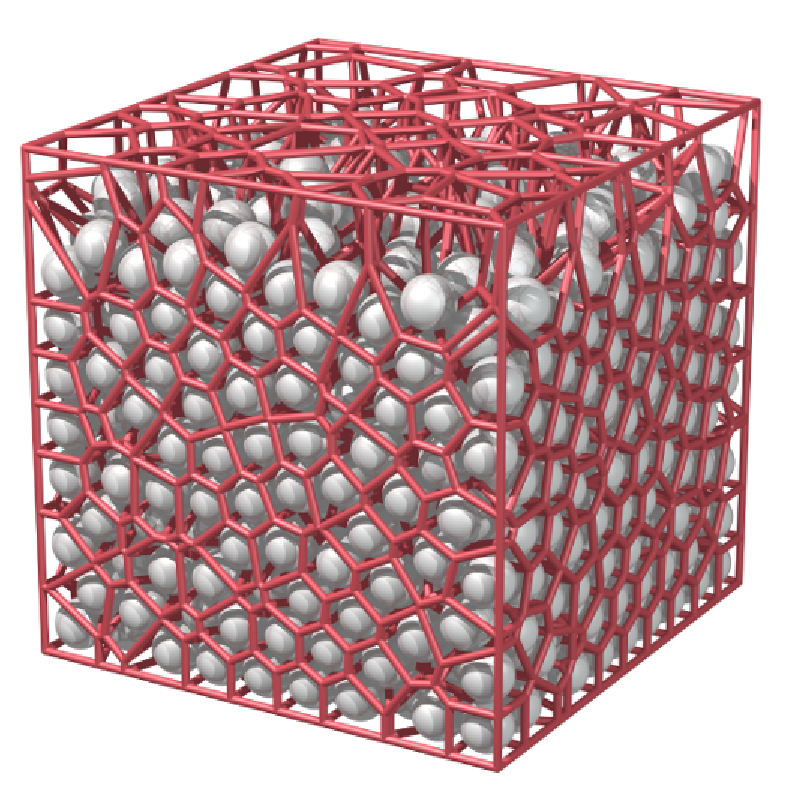
\includegraphics[width=0.45\textwidth]{voro3d_small}}
	\caption{Voronoi decomposition.}
	\label{fig:voro}
\end{figure}

Another method to select construct the bond graph is the Voronoi decomposition (see \FigureRef{fig:voro}). The space is split in cells, one per particle. The cell of the particle P contains all the points closer to P than to any other particle. In 2D the Voronoi cell is a convex polygon sharing a side with its neighbours. In 3D, the surface of a Voronoi cell is composed of flat polygons shared between two particles. A vertex is equidistant from more than two particles. If two particles share a surface and that the line that join them intersects this surface, we define the particles as bonded.

However, we have to keep in mind that the Voronoi decomposition can be very unstable. Around high order vertices (4 or more equidistant particles), even a very slight perturbation of the sites may change the diagram topology and therefore the bond graph~\citep{weller1997stability, ReintenWolde1996, Williams2007}. Some authors propose modified versions of the Voronoi decomposition with better stability. Each of these versions has a goal, for example selecting only the stable bonds~\citep{weller1997stability} or finding the high order vertices~\citep{Williams2007, rycroft2007multiscale} despite their instability.

Contrary to the maximum bond length method, the Voronoi decomposition potentially yields very anisotropic cells~\citep{Schroder-Turk2010}. Considering far-apart particles as bonded may obfuscate the meaning of local symmetries. Thus, in this thesis we prefer the maximum bond length method.

\subsection{Inherent structure}

We have seen in \SectionRef{sec:config_vib} that in dense phases, it is possible to decompose the entropy $S$ of the system between a configurational part $S_c$ and a vibrational part $S_v$. Conceptually, a particle vibrates around a (regular or not) lattice position. The structure we are interested in is this "lattice". Unfortunately, the thermal motion of the particles can alter both topology and geometry of the bond network, obscuring the underlying structure. 

Stilliger and co-workers~\citep{Stillinger1982, Stillinger1984} propose to quench numerically a given configuration, making each particle follow the steepest-descent path locally available on the energy landscape. After this process each particle sits at its local potential energy minimum. Performing the structural analysis on this "inherent structure" gives much sharper results (see \FigureRef{fig:inherent}).

Stilliger's method can be applied only to systems with a potential energy, not to athermal systems like hard spheres. For these systems, other methods were proposed, like fast inflation of the volume of the particle~\citep{Stillinger1985, berthier2009gtd} or averaging positions on short time~\citep{santen2000absence}.

One can argue that an experimental method giving the short-time average of the positions of the particles would yield in fact the inherent structure of the system. Because of the acquisition time, confocal microscope may already give such information.

\begin{figure}
	\centering
	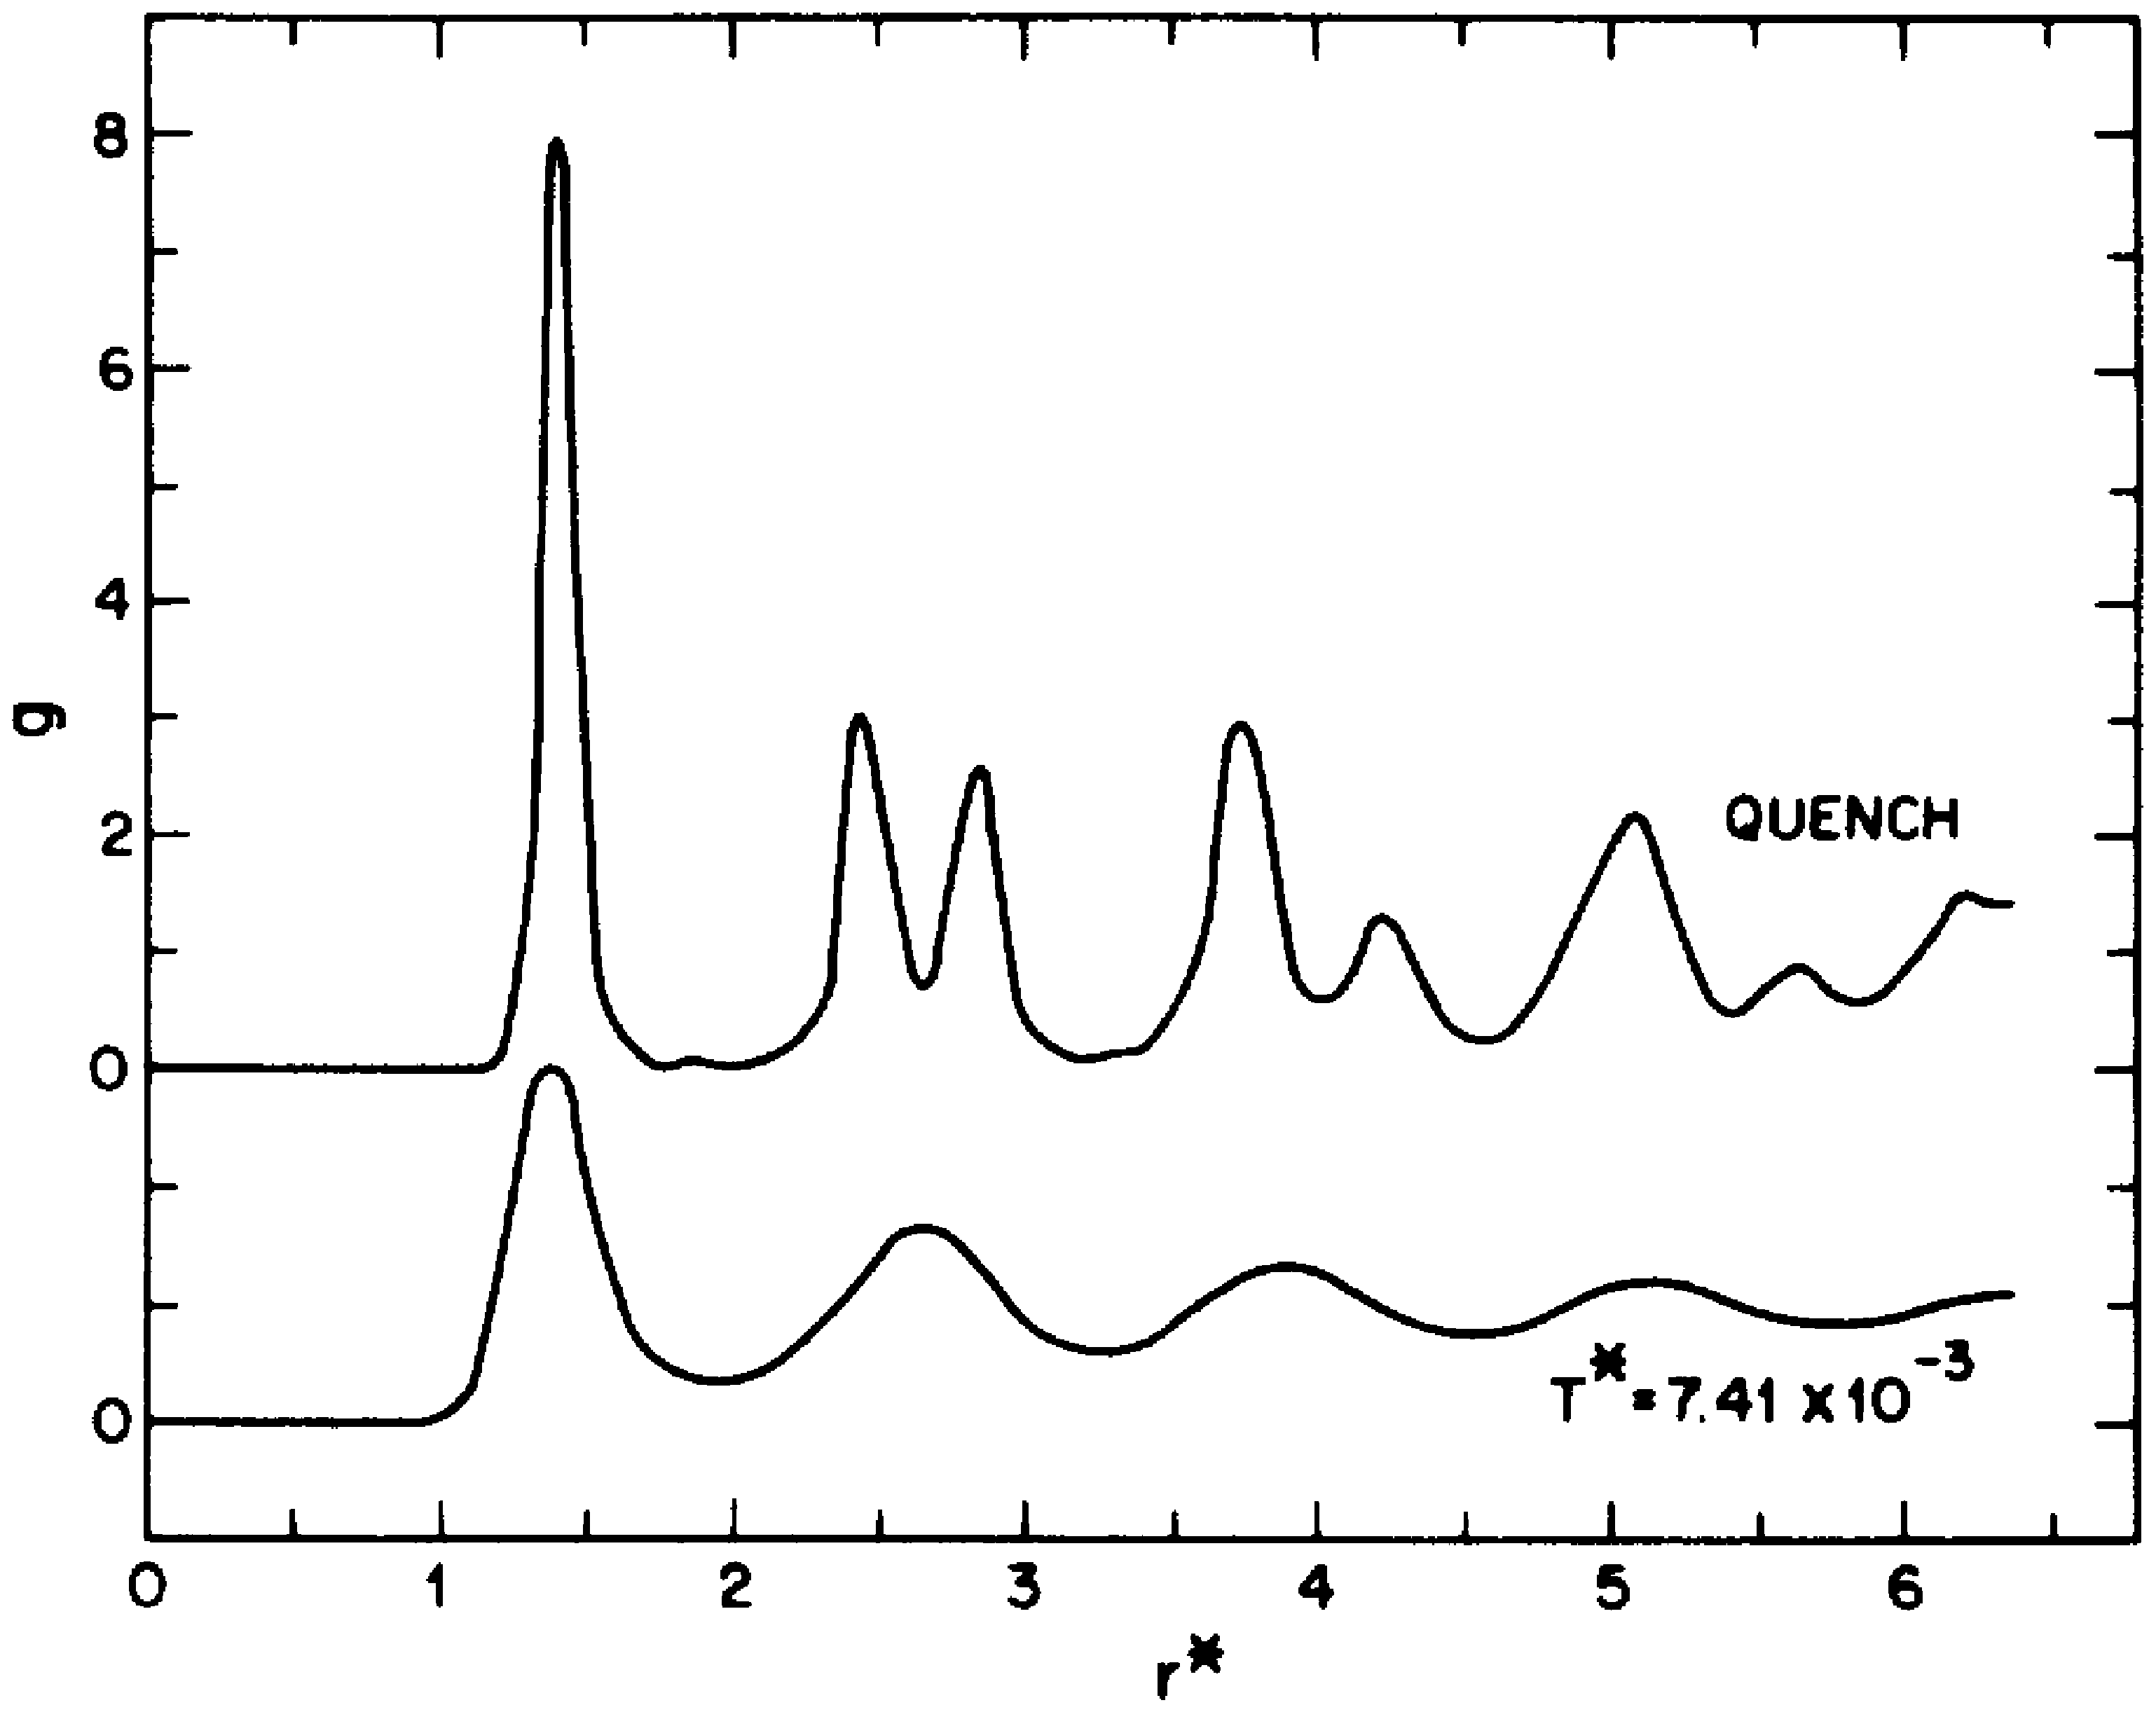
\includegraphics[width=0.6\textwidth]{steepest_descent}
	\caption{Radial distribution function of a fluid (Gaussian core model in 2D) and the corresponding "inherent structure". Source \ReferenceRef{Stillinger1982}.}
	\label{fig:inherent}
\end{figure}

\section{Topology of the bond network}

A first way to look for structure is to consider only the topology of the bond graph. Because topology is invariant by continuous deformations, topological methods give discrete variables, changing in a discontinuous manner in time and space.

\subsection{Coordination number}

Once the bond network established, it is straightforward to count the number of bonds per particle, also called coordination number. The coordination number is a very simple but rough way to categorise local structures. Actually, most of the particles in a system of monodisperse isotropic repulsing disks system will have 6 neighbours, even if they are not crystalline (see \FigureRef{fig:coordination}). The same is true in for repulsive spheres who have almost always 12 neighbours but various types of crystalline or non-crystalline orders.

\subsection{Voronoi cell shape}

\subsubsection{2D: Geometrical defects}

The importance of geometrical defects (voids) in 2D melting of a hexagonal crystal of monodisperse hard discs has been emphasised by Glaser and Clark~\citep{Glaser1990}. To emphasise the defects to the perfect triangular paving of the plan, they systematically decimate the bond graph obtained by Voronoi decomposition by removing the bonds longer than the maximum bond length. This reveals patches of triangles (crystal-like) and ladder-like clusters of squares or higher order polygons (defects) (see \FigureRef{fig:defects}).

\begin{figure}
	\centering
	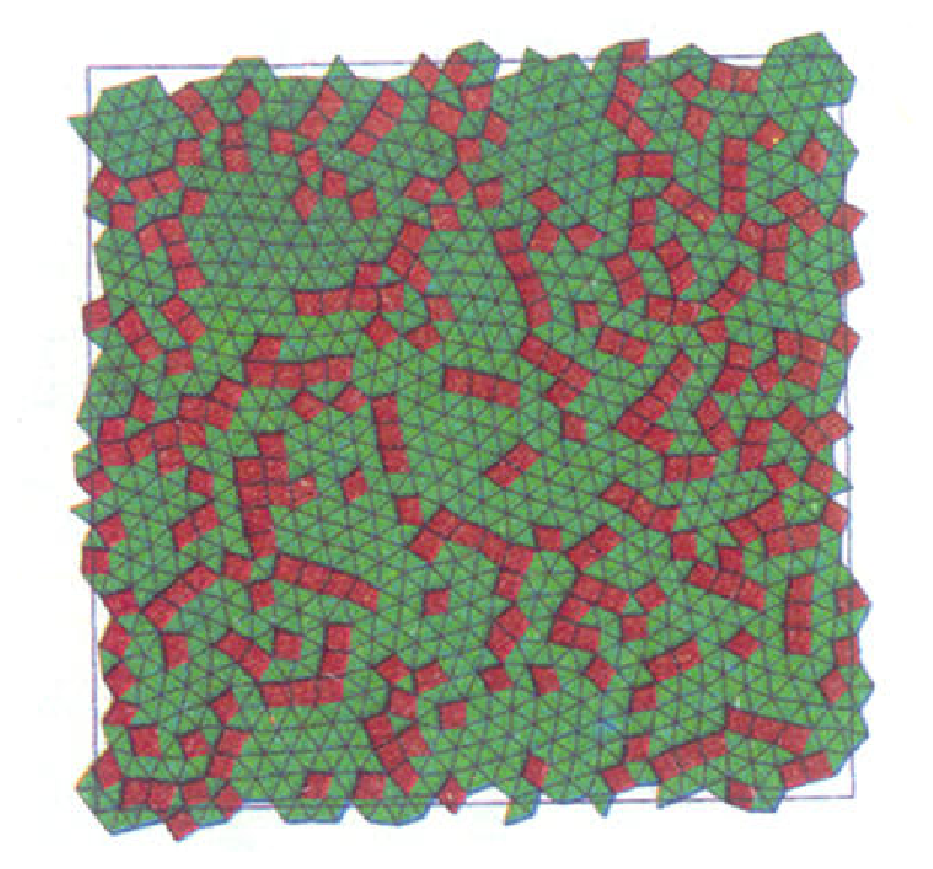
\includegraphics[width=0.6\textwidth]{defects}
	\caption{Bond network of a repulsive 2D liquid obtained by decimated Voronoi decomposition (see text). Triangles of bonds are shown in green, polygons of 4 or more bonds (defects) are shown in red. Source \ReferenceRef{Glaser1990}.}
	\label{fig:defects}
\end{figure}

\subsubsection{3D: Voronoi signature}

The shape of the Voronoi cell was often used in 3D to identify local structure~\citep{Duijneveldt1992, Cape1981, Hsu1979a, Nose1986, tanemura1977geometrical}. It is customary to define the signature of a Voronoi polyhedron as a set of integers $(n_3 ,n_4 ,n_5 ,\ldots)$, where $n_l$ is the number of $l$-sided faces of the polyhedron. For example, the Voronoi polyhedron of a perfect \ac{FCC} structure, the rhombic dodecahedron that has twelve lozenge-shaped faces, is denoted by $(0, 12, 0, 0, \ldots)$, while the Voronoi polyhedron of a particle in a \ac{BCC} structure, is denoted by $(0, 6, 0, 8, 0, \ldots)$ (six squares, eight hexagons).

In practice, the Voronoi signatures of the particles in a crystal will be modified by the thermal vibrations (see \FigureRef{fig:voroCell}). For instance, the characteristic Voronoi polyhedron of the \ac{FCC} lattice, the rhombic dodecahedron, will be removed by the tiniest thermal motion. Of the 14 vertices of the rhombic dodecahedron there are six where four faces meet. Any thermal motion will make these fourfold vertices break up into sets of threefold vertices connected by short edges. The result is that a variety of polyhedra such as $(0,3,6,4)$, $(0,3,6,5)$, $(0,4,4,6)$, $(0,4,4,7)$ occur in a thermally equilibrated \ac{FCC} crystal. Hence, Voronoi signatures can only be used in a statistical sense to identify solid-like particles.

\begin{figure}
	\centering
	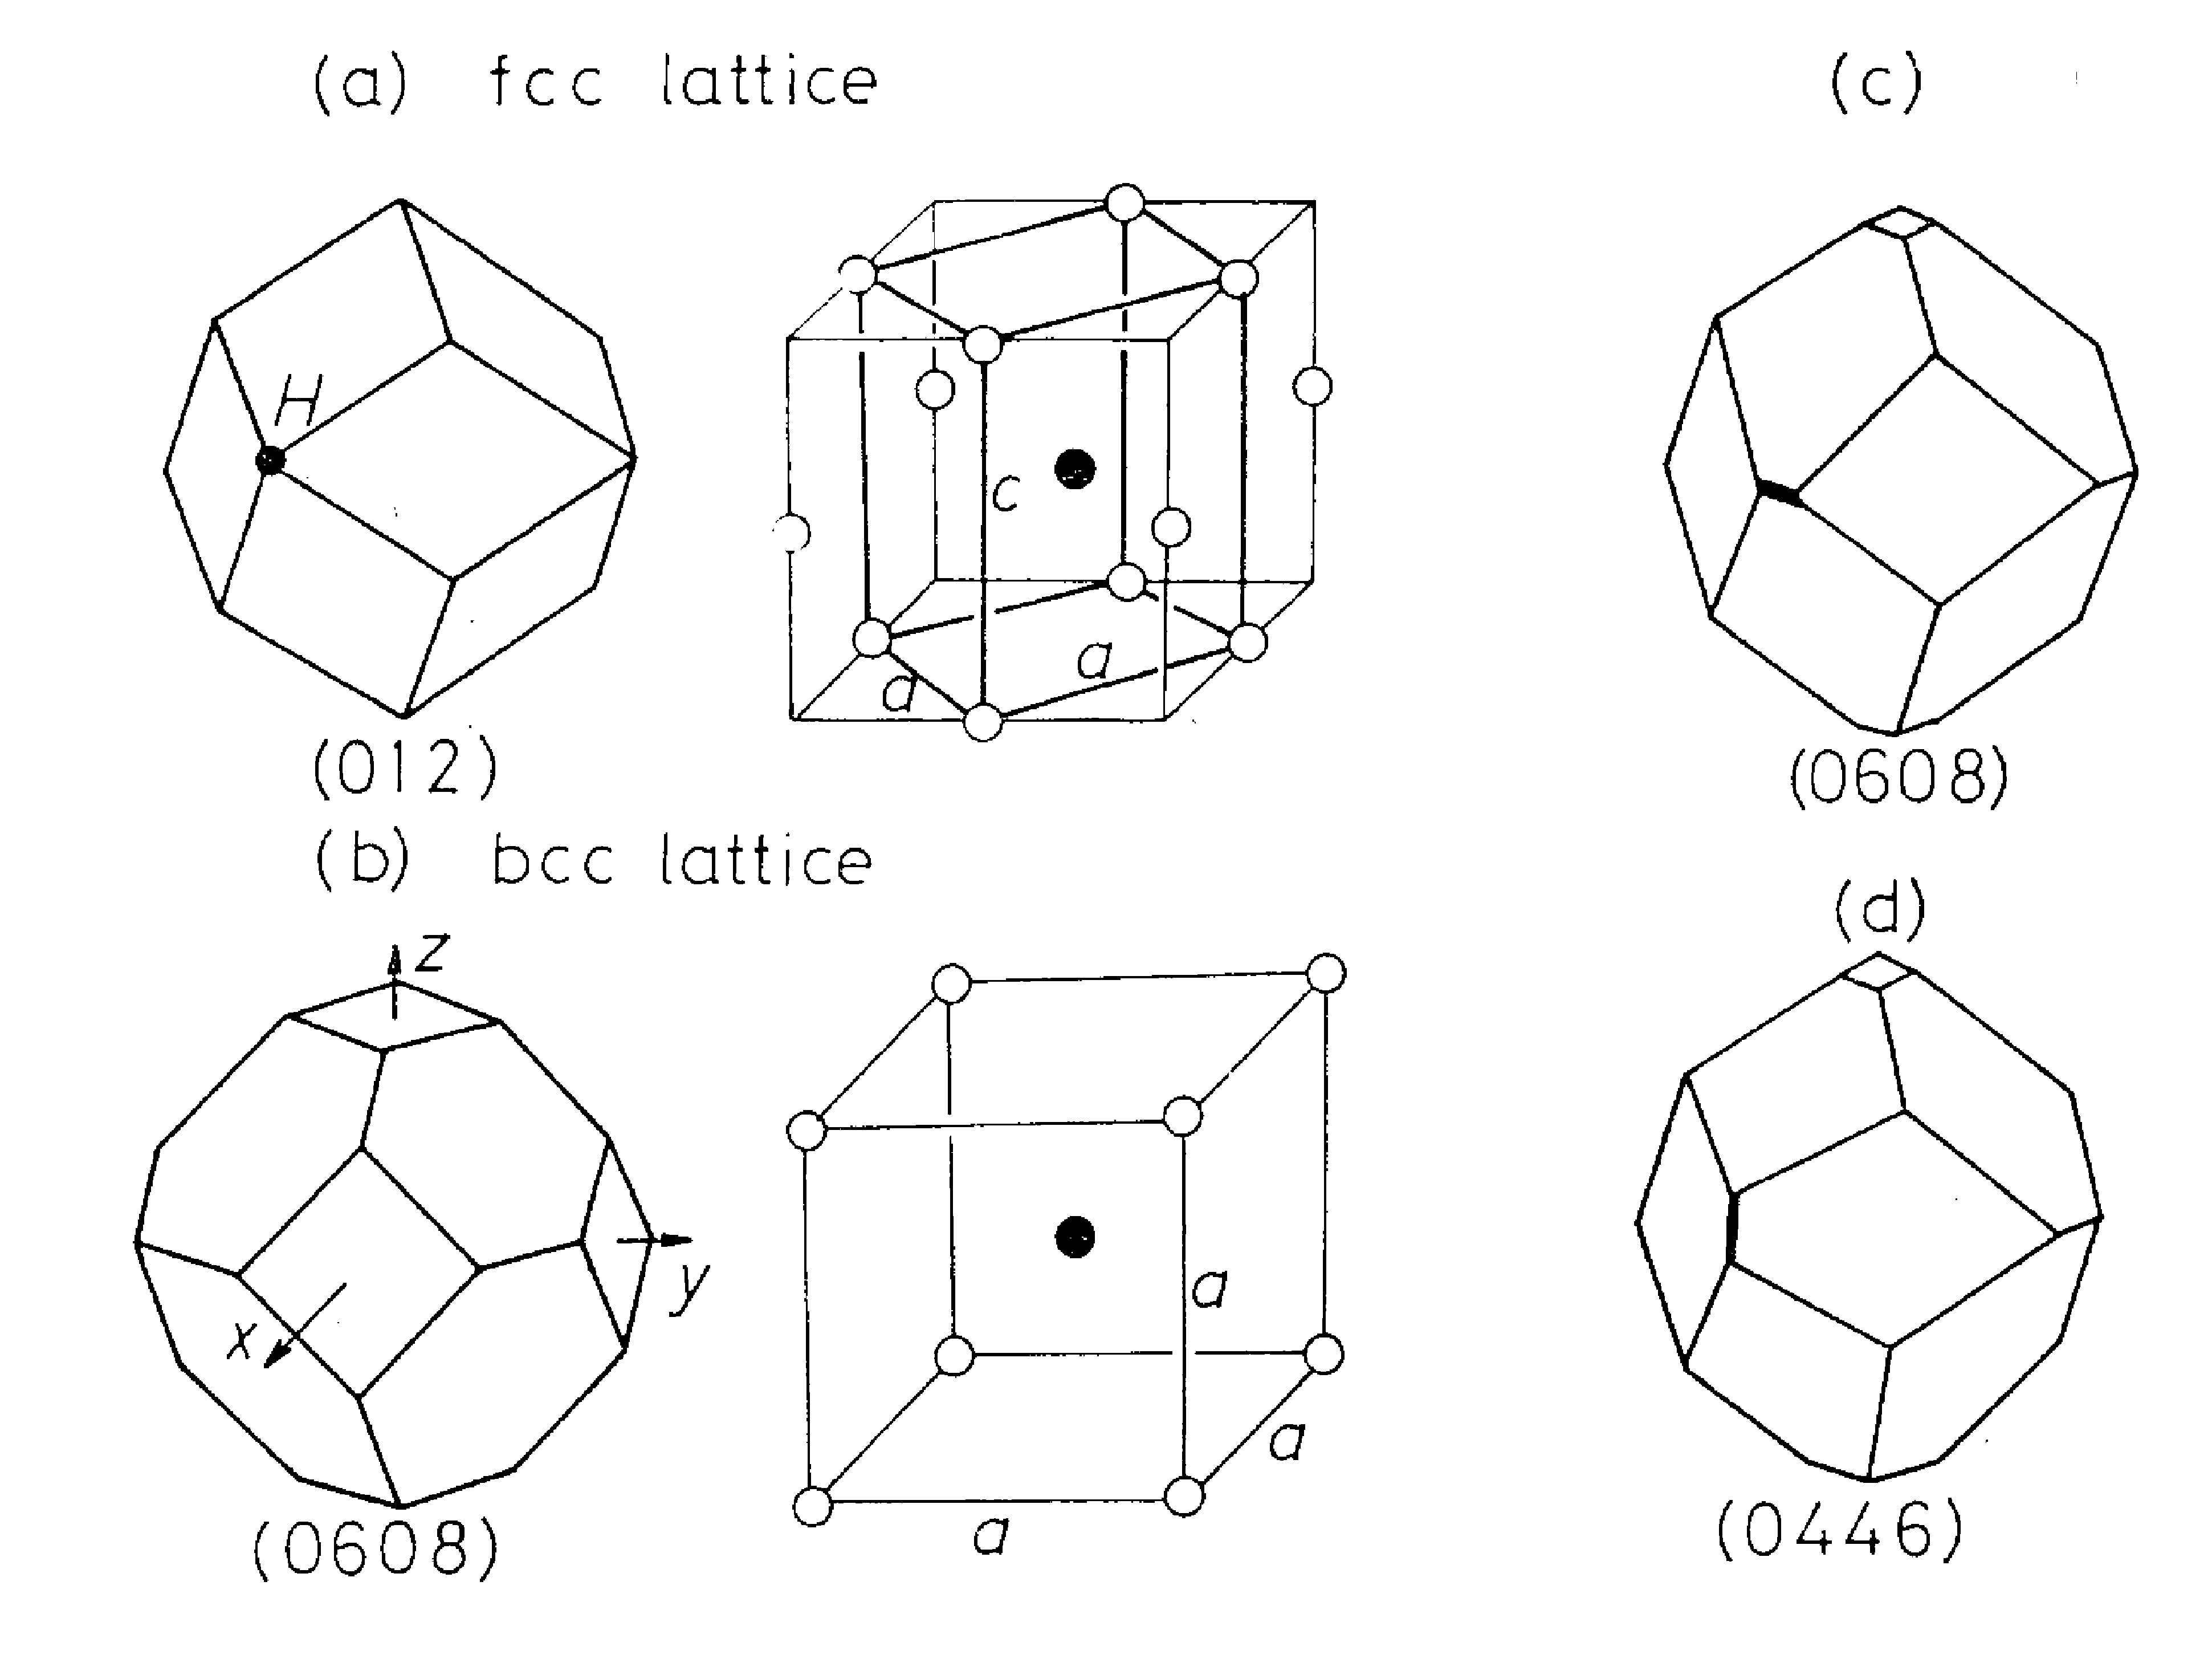
\includegraphics[width=0.6\textwidth]{voro_cell}
	\caption{Topological relations between $(0,6,0,8)$ and $(0,4,4,6)$ polyhedra. (a) \acs{FCC} lattice, (b) \acs{BCC} lattice. Black circles are centred atoms of respective Voronoi polyhedra. If the parallelepiped indicated by bold lines in (a) is compressed from top to bottom, it turns out to the unit cell of (b). (c) $(0,6,0,8)$ polyhedron, (d) $(0,4,4,6)$ polyhedron. If the horizontal bold line is replaced by the vertical, the $(0,6,0,8)$ polyhedron changes to the $(0,4,4,6)$ polyhedron and vice versa. Source \ReferenceRef{tanemura1977geometrical}}
	\label{fig:voroCell}
\end{figure}

\subsection{Common neighbours analysis}
\label{sec:commonNgb}

We know that any given particle has almost always 12 neighbours. Topological differences come when looking at the neighbours of the neighbours. Following this idea, \citet{Honeycutt1987} looked at the common neighbours of two particles A and B. They give 4 indices to characterise the pair:
\begin{enumerate}
	\item Are A and B bounded? (1 or 2)
	\item Number of neighbours common to A and B
	\item Number of bonds between the common neighbours
	\item Distinguishing between different arrangements of the bonds.
\end{enumerate}

They focus on two types of pairs: the 1551 and the 2331. The 1551 pair corresponds to two neighbouring particles with five common neighbours that form a pentagon of bonds. The 2331 pair corresponds to two particles that are not neighbours but have three common neighbours that form a triangle of bonds. The two types of pairs are characteristic of icosahedral ordering (see \FigureRef{fig:commonNgb}). 1421 and 1422 are characteristic of crystals.

\begin{figure}
	\centering
	\subfloat[1551-pair]{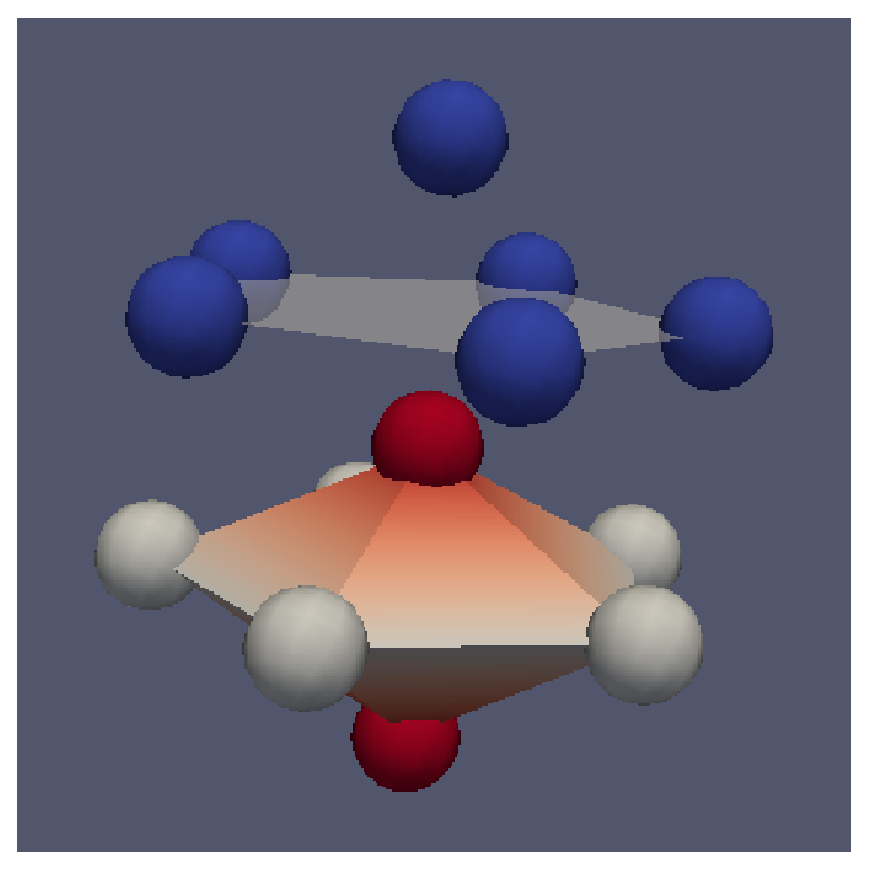
\includegraphics[width=0.3\textwidth]{ico_13_1551}}\quad
	\subfloat[2331-pair]{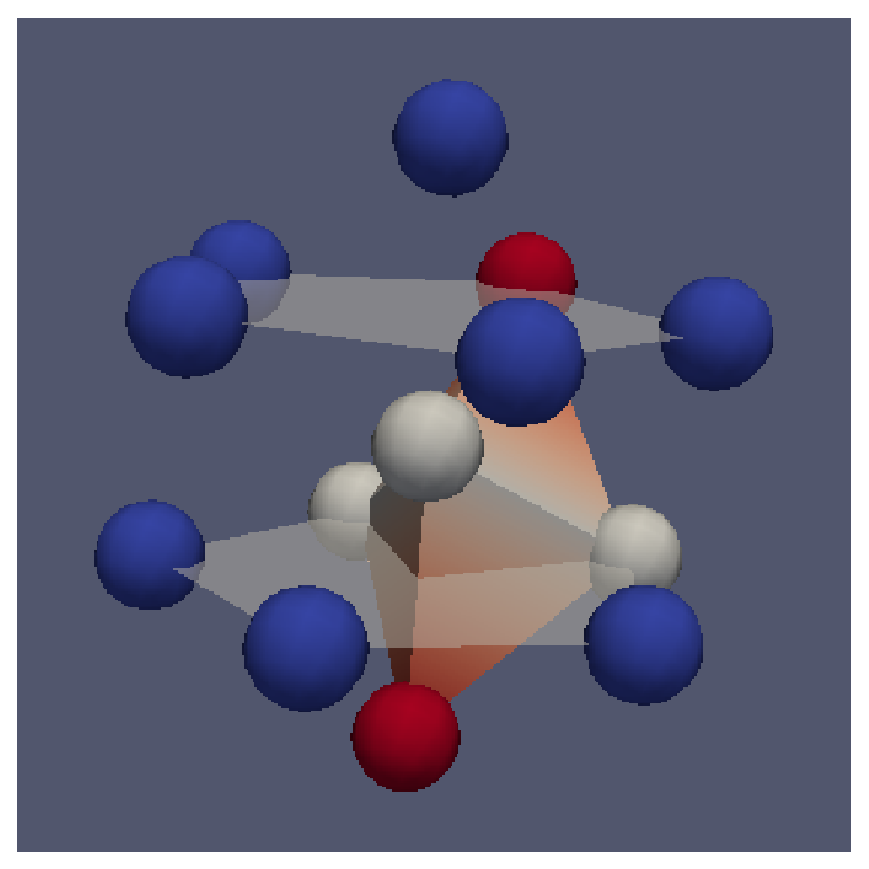
\includegraphics[width=0.3\textwidth]{ico_13_2331}}
	\caption{Characteristic pairs of 13-particles icosahedron. Red particles are the particles of the pair. White particles are the common neighbours. Blue particles are the rest of the icosahedron. Pairs are name in the common neighbour analysis terminology (see \SectionRef{sec:commonNgb}). Note that their are more than one pair of each type in the icosahedron.}
	\label{fig:commonNgb}
\end{figure}

\subsection{Topological cluster classification}
\label{sec:TCC}

The \acf{TCC} is a generalisation of the common neighbour analysis by Williams~\citep{Williams2007}. Its goal is to identify simple clusters inside a bulk phase. The selected clusters are the Morse clusters~\citep{doye1995effect} of less than 13 particles and the 13 atom clusters found in an \ac{FCC} and an \ac{HCP} crystal phase. One first search for 3, 4 and 5 membered shortest path (SP) rings~\citep{Franzblau1991}. A letter is then assigned to the ring depending on the number of particles bonded to all the ring's members: a for the ring alone; b if only one particle is bonded to all the ring's members; c for two particles, one on each side of the ring. In practice the SP5c and SP3c clusters corresponds to Jonsson and Andersen's 1551 and 2331 pairs respectively. The SPnx clusters are then combined to form larger clusters. A full icosahedral cluster contained 12 overlapping SP5c clusters is composed of two SP5c clusters sharing one spindle particle (see \FigureRef{fig:commonNgb}).

Analysing the results is a simple matter to record the atoms which form the various clusters. If some of the clusters have been identified multiple times this can be checked for and corrected later. However the reporting of population levels for the various clusters opens up choice and ambiguity. This is because any given atom may be a member of several different clusters. Williams reports the population levels in the following manner. If an atom is a member of a cluster and also a member of a different cluster which has more atoms it is only identified with the larger cluster. An atom may be a member of two clusters consisting of the same number of atoms, in this case the atom is reported as being a member of both clusters if it is not a member of any larger clusters. Using this approach we can construct a histogram of the net population levels for the various clusters (see \FigureRef{fig:tcc} for an example in hard sphere fluid).

\begin{figure}
	\centering
	\includegraphics[width=0.8\textwidth]{histTCC}
	\caption{A histogram of the net population levels for the various clusters in a hard sphere fluid. Source \ReferenceRef{Williams2007}.}
	\label{fig:tcc}
\end{figure}

\subsection{Limits of topological approaches}

Analysis of the topology of the bond network gives discrete categories of structures. Thus, one observes discrete jumps from one category to another both in time and in space. A common example is a cluster of particles that is detected alternatively in the categories A and B when followed in time. Is this cluster A or B? Do we need to create a new category A+B? How to describe the time correlation of these discrete structures? And how can we characterize the spatial extent of a collection of structures?

\section{Bond orientational order}
\label{sec:boo}

To go further into local structure analysis, one need to take into account both the topology of the bond network and its local symmetry.

\subsection{Hexatic order parameter - \texorpdfstring{$\psi_6$}{psi6}}

\begin{figure}
	\centering
	\includegraphics[width=0.8\textwidth]{coordination}
	\caption{Relationship between dynamic heterogeneity, medium-range crystalline order, and topological defects for a quasi-2D driven granular matter system. (a) Particle trajectory during $t_0 < t < t_0 +\tau_\alpha$ ($t_0$: arbitrary). (b) Spatial distribution of the time-averaged ($t_0 < t < t_0 +\tau_\alpha$) bond-orientational order parameter $\psi_6$. (c) Spatial distribution of the coordination number Z at $t = t_0$. Clusters of particles with high crystalline order in (b) and the corresponding region in (a) and (c) are circled for a guide to the eye. Note that almost all the particles have a coordination number $Z=6$ but display a wide range of $\psi_6$. Source \ReferenceRef{watanabe2008}}
	\label{fig:coordination}
\end{figure}

In 2D, it is possible to define the hexatic order parameter~\citep{Nelson1979, Binder2002, Hamanaka2006, kawasaki2007cbd} $\psi_6$ to detect the degree of six-fold symmetry around given particle $i$:
\begin{equation} 
	\psi_{6}^{i}=\frac{1}{n_i}\sum^{n_i}_{k=1}e^{j6\theta^i_{k}} 
\end{equation}
where $n_i$ is the number of nearest neighbours of particle $i$, and $\theta^i_k$ is the angle between $\vec{r}_{ik} = \vec{r}_k - \vec{r}_i$ and the x axis, where particle $k$ is a neighbour of particle $i$ ($j$ is the imaginary number). $\psi_{6}^{i}=1$ means the perfect hexagonal arrangement of six nearest-neighbour particles around particle $i$ and $\psi_{6}^{i}=0$ means a random arrangement.

One can follow the averaged order parameter $\psi_6= \langle \psi^{i}_{6} \rangle$ to study the liquid to hexatic to crystal phase transition, or the link between local order and dynamics (see \FigureRef{fig:coordination}). Moreover, $\psi_{6}^{i}$ is a continuous, local order parameter, defined at the particle level. It is then possible to define its spatial correlation $g_6(r) = |\langle \psi_6^k \psi_{6}^{l} \rangle|$, with $r = |\vec{r_l} - \vec{r_k} |$. $g_6(r)$ should decay to zero if the hexatic order is only local.

Steinhardt's bond orientational order (BOO)~\citep{steinhardt1983boo} is the generalised analog in 3D of the hexatic bond orientational order. To understand its meaning we need to explain some mathematics.

\subsection{Spherical harmonics}

\begin{figure}
	\centering
	\subfloat[$\ell=4$, $m=0$]{\label{fig:sh4-0}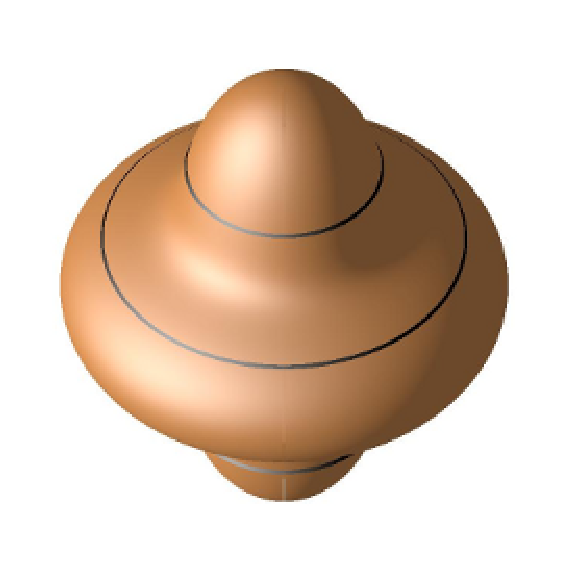
\includegraphics[width=0.25\textwidth]{sh4-0}}
	\subfloat[$\ell=4$, $m=4$]{\label{fig:sh4-4}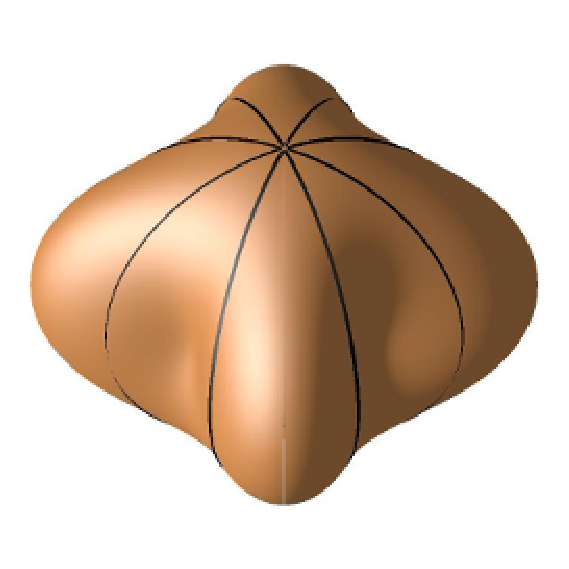
\includegraphics[width=0.25\textwidth]{sh4-4}}
	\subfloat[$\ell=10$, $m=10$]{\label{fig:sh10-10}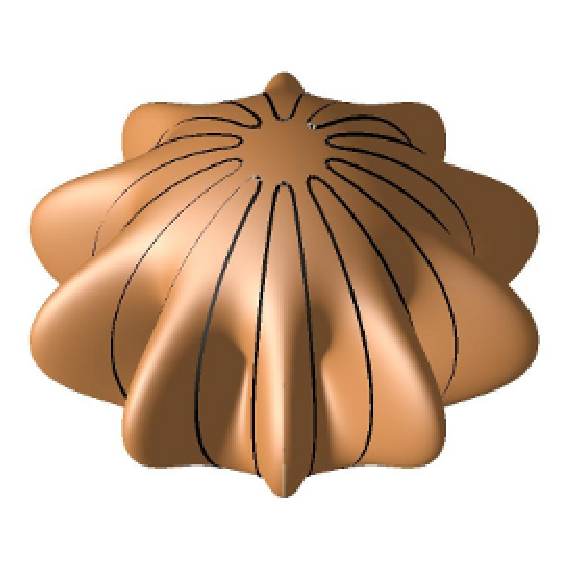
\includegraphics[width=0.25\textwidth]{sh10-10}}\\
	\subfloat[$\ell=6$, $m=0$]{\label{fig:sh6-0}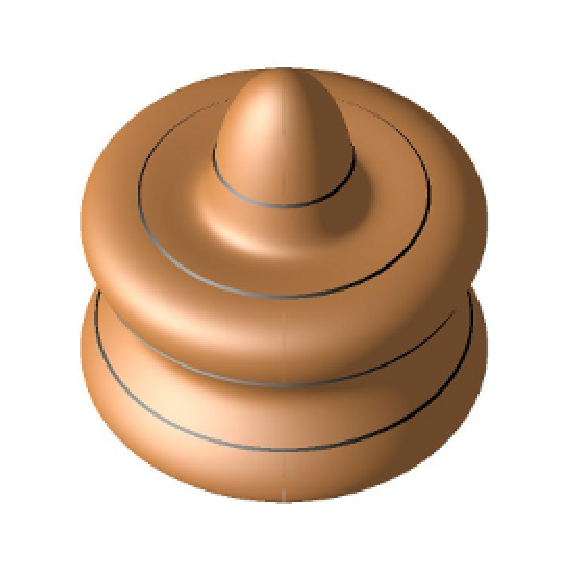
\includegraphics[width=0.25\textwidth]{sh6-0}}
	\subfloat[$\ell=6$, $m=3$]{\label{fig:sh6-3}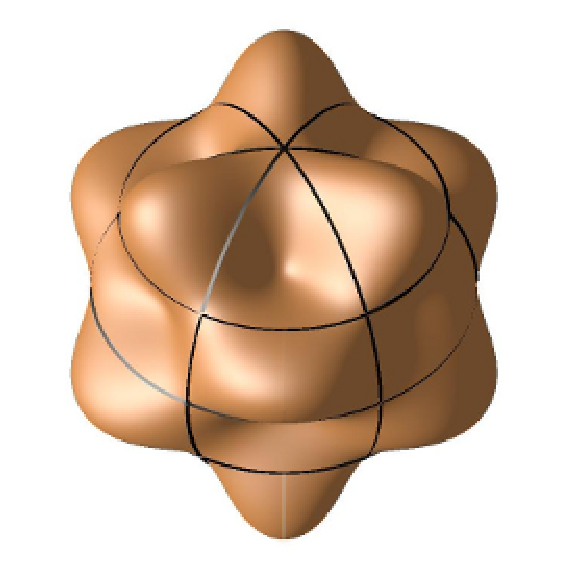
\includegraphics[width=0.25\textwidth]{sh6-3}}
	\subfloat[$\ell=6$, $m=5$]{\label{fig:sh6-5}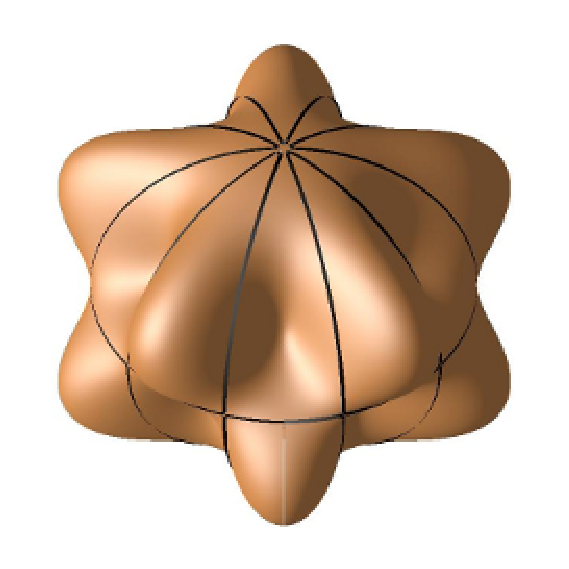
\includegraphics[width=0.25\textwidth]{sh6-5}}
	\subfloat[$\ell=6$, $m=6$]{\label{fig:sh6-6}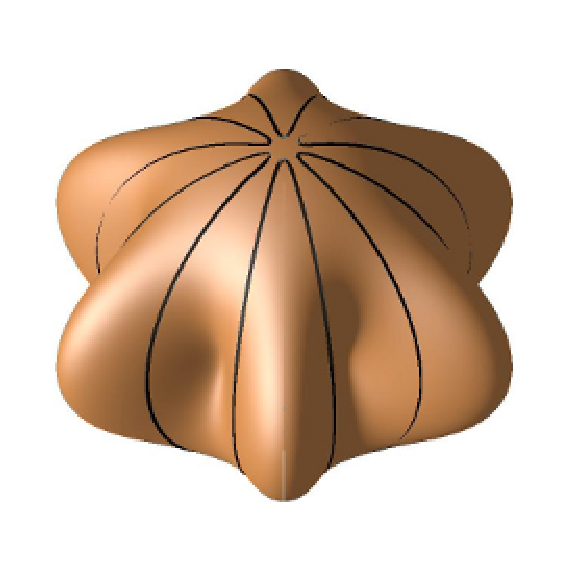
\includegraphics[width=0.25\textwidth]{sh6-6}}
	\caption{Spherical Harmonics at various order and degree. Note how a \acs{FCC} cluster can be approximated by the sum of \subref{fig:sh6-6} for the hexatic plane and \subref{fig:sh6-3} for the upper and lower planes. In the same way the two 5-particle rings of an Icosahedron look like \subref{fig:sh6-5} whereas the spindle atoms can be described by \subref{fig:sh6-0}. \subref{fig:sh10-10} is common to both Icosahedron and Dodecahedron. Source \ReferenceRef{AllenMcNamara}.}
	\label{fig:SphericalHarmonics}
\end{figure}

\begin{figure}
	\centering
	\def\svgwidth{0.6\textwidth}\input{earth_spectrum.pdf_tex}
	\caption{Spectrum of the earth topography. y axis is in meters. The curve is decreasing, meaning that the lower degrees (long wavelength) are of larger amplitude than the higher degrees (short wavelength). Source \ReferenceRef{Vigny}.}
	\label{fig:earth_spectrum}
\end{figure}

The spherical harmonics $Y_{\ell m}(\theta,\phi)$ are an infinite orthogonal base of functions. All fields (solution of Laplace equation) on a sphere can be decomposed into spherical harmonics. $\ell \geq 0$ indicates the order of symmetry. $m$, with $-\ell \geq m \geq \ell$, indicates the orientation with respect to a referent set of orthonormal axes. \FigureRef{fig:SphericalHarmonics} represents a few spherical harmonics.

Let us give a concrete example: earth topology. In first approximation, planet earth is a sphere, but this sphere has some roughness (Mount Fuji is a roughness of 3,776 m compared to sea level). We note $h(\theta,\phi)$ the altitude of the surface of the earth compared to sea level at latitude $\theta$ and longitude $\phi$. This field can be decomposed into an infinite sum of spherical harmonics:
\begin{equation} 
h(\theta,\phi) = \sum_{\ell=0}^{\infty} \sum_{m=-\ell}^{\ell} q_{\ell m} Y_{\ell m}(\theta,\phi)
\end{equation}
The $q_{\ell m}$ coefficients are complex numbers. The spectrum of the field $h(\theta,\phi)$ is the sequence of number $SP_\ell$ giving the amplitude of the term $\ell$ in the spherical harmonics decomposition (see \FigureRef{fig:earth_spectrum}).
\begin{equation} 
	SP_\ell = \sqrt{\frac{1}{4\pi} \sum_{m=-\ell}^{\ell} |q_{\ell m}|^2 } 
\end{equation}

Terms with small $SP_\ell$ can be neglected to give an approximation of the field $h(\theta,\phi)$. The more terms that are left, the better the approximation(see \FigureRef{fig:earthApprox})

\begin{figure}
	\centering
	%\subfloat[$\ell=0$]{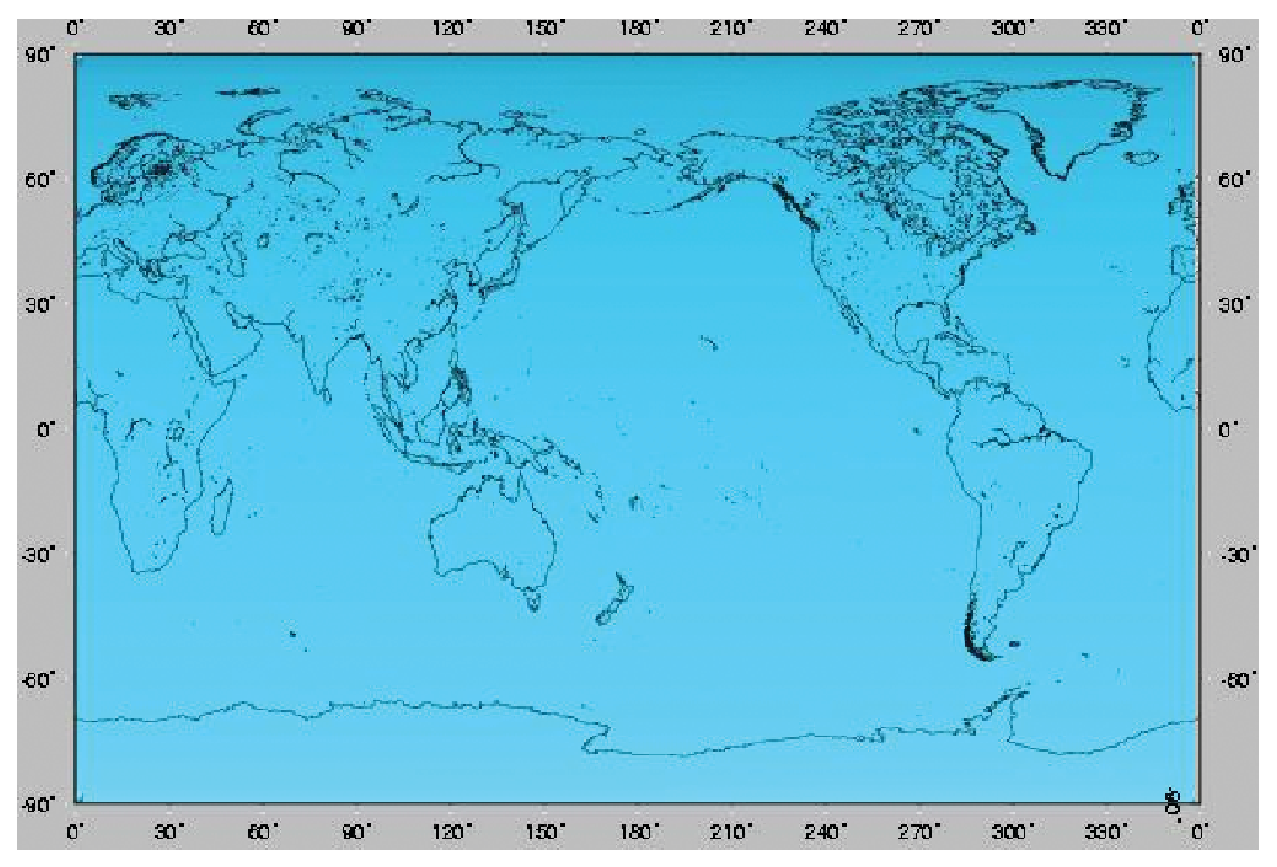
\includegraphics[width=0.3\textwidth]{earth_l0}}
	\subfloat[$\ell=1$]{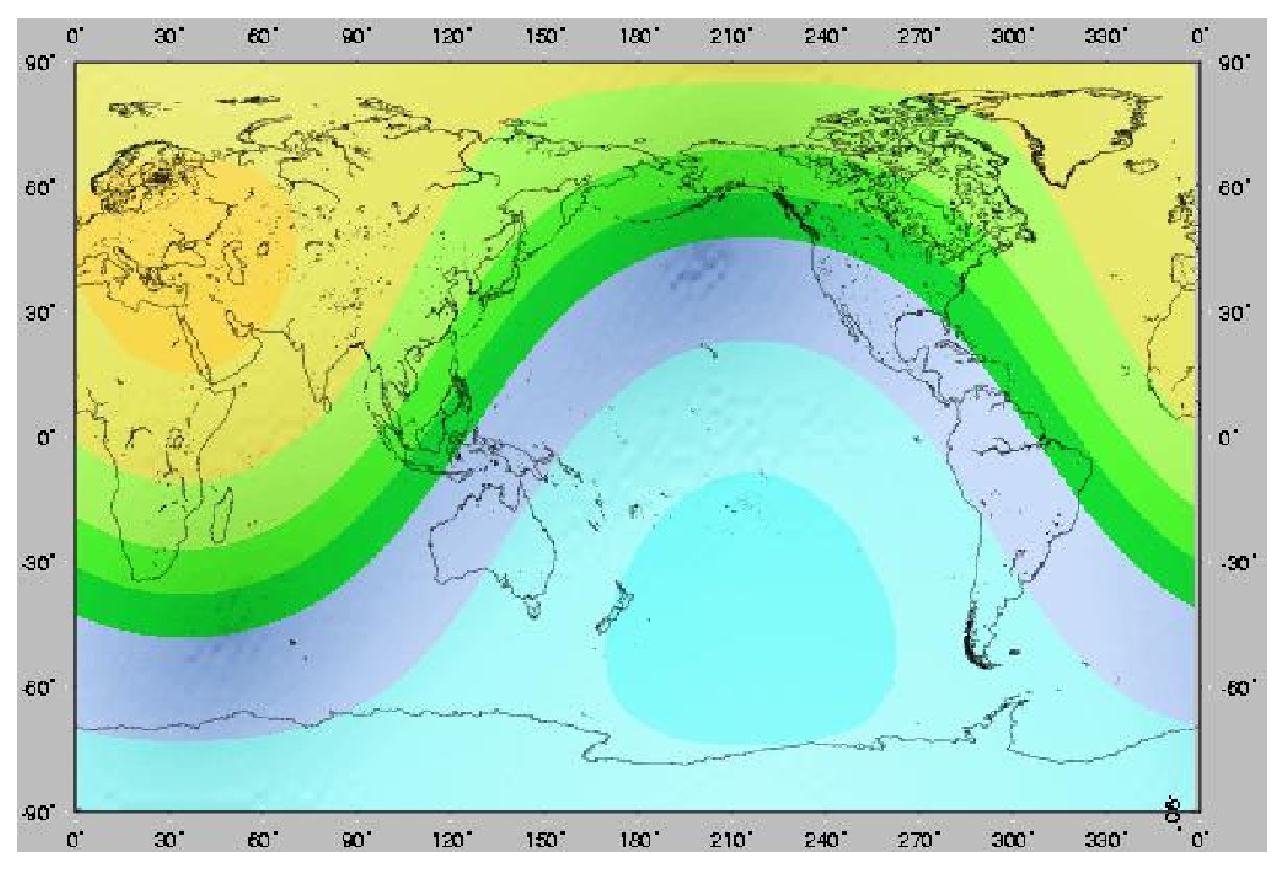
\includegraphics[width=0.3\textwidth]{earth_l1}} 
	\subfloat[$\ell=2$]{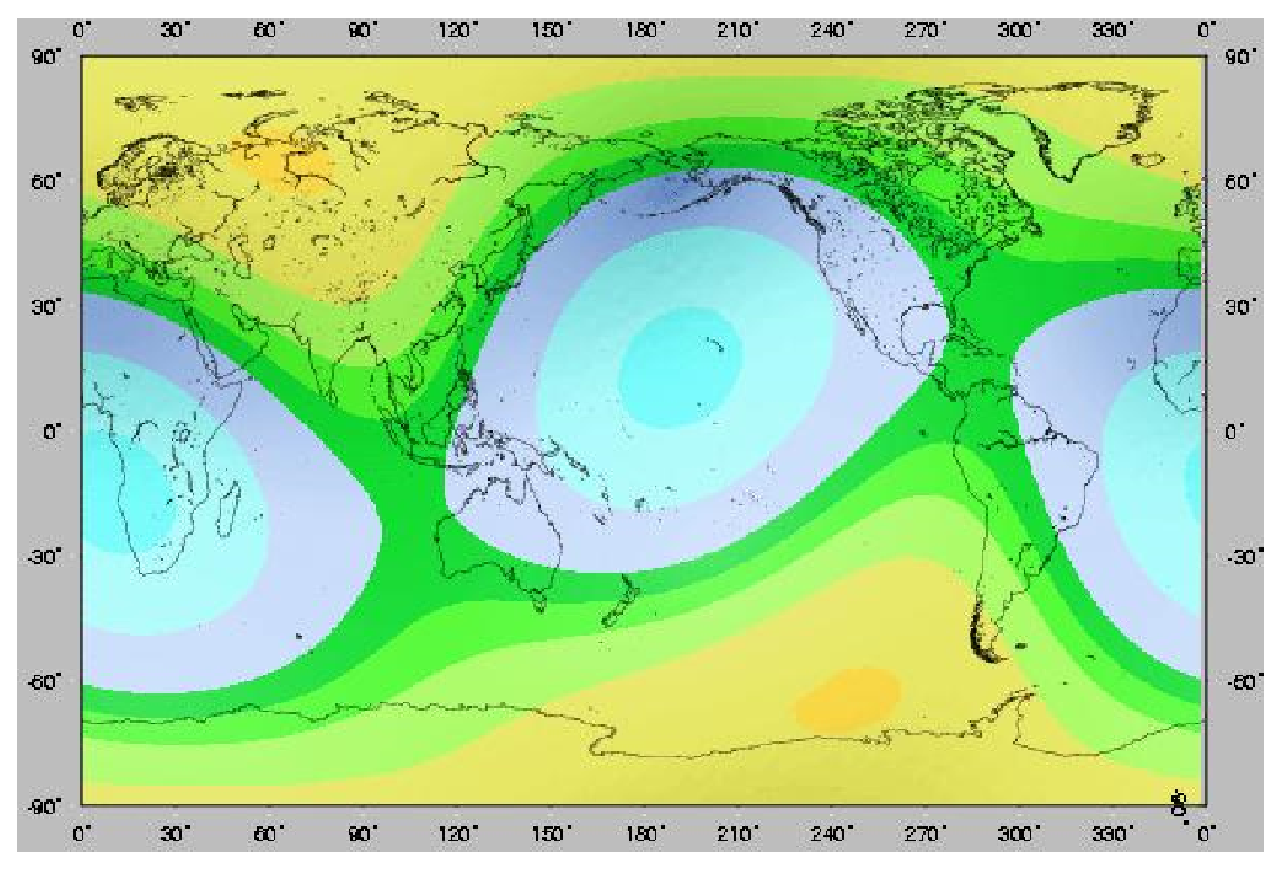
\includegraphics[width=0.3\textwidth]{earth_l2}} 
	\subfloat[$\ell=3$]{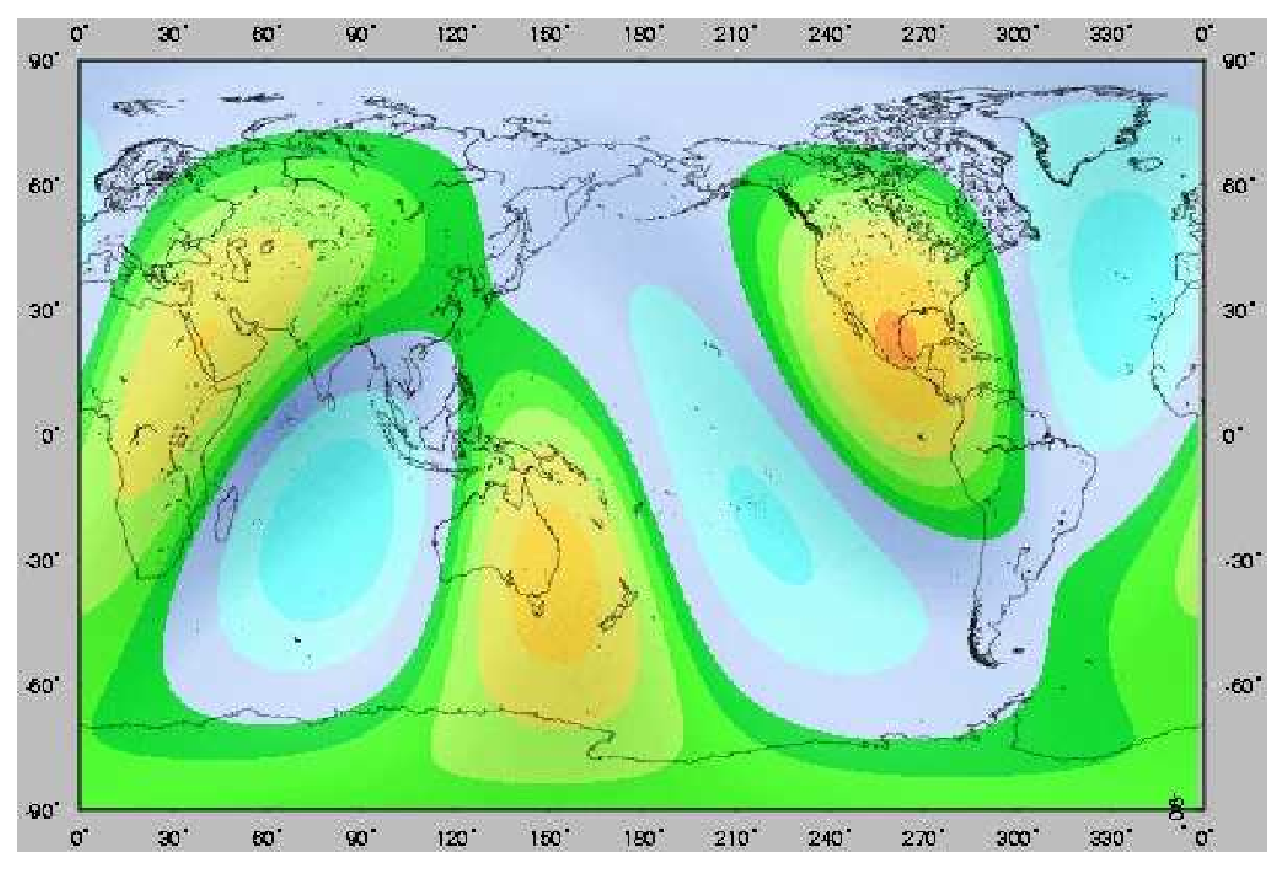
\includegraphics[width=0.3\textwidth]{earth_l3}}\\
	\subfloat[$\ell=4$]{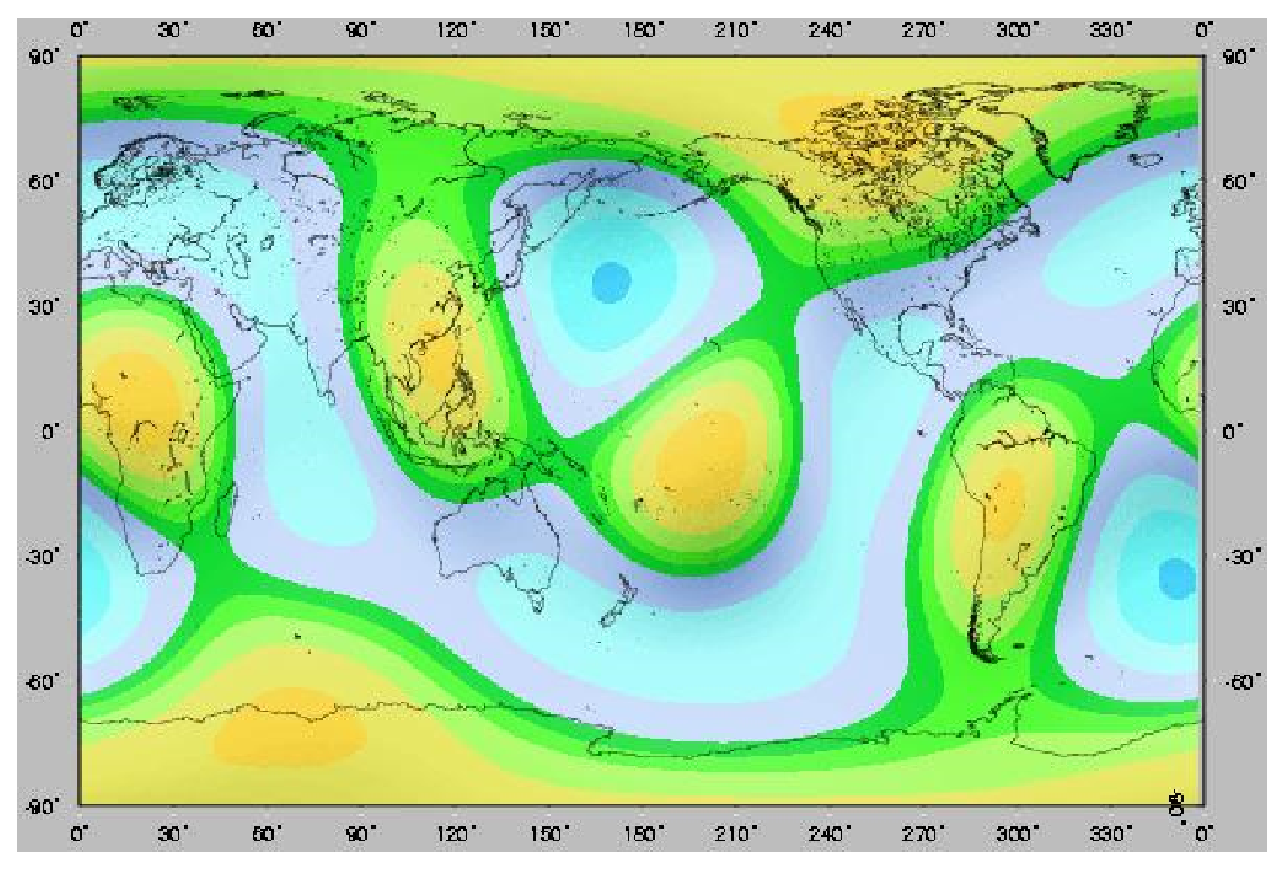
\includegraphics[width=0.3\textwidth]{earth_l4}} 
	\subfloat[$\ell=5$]{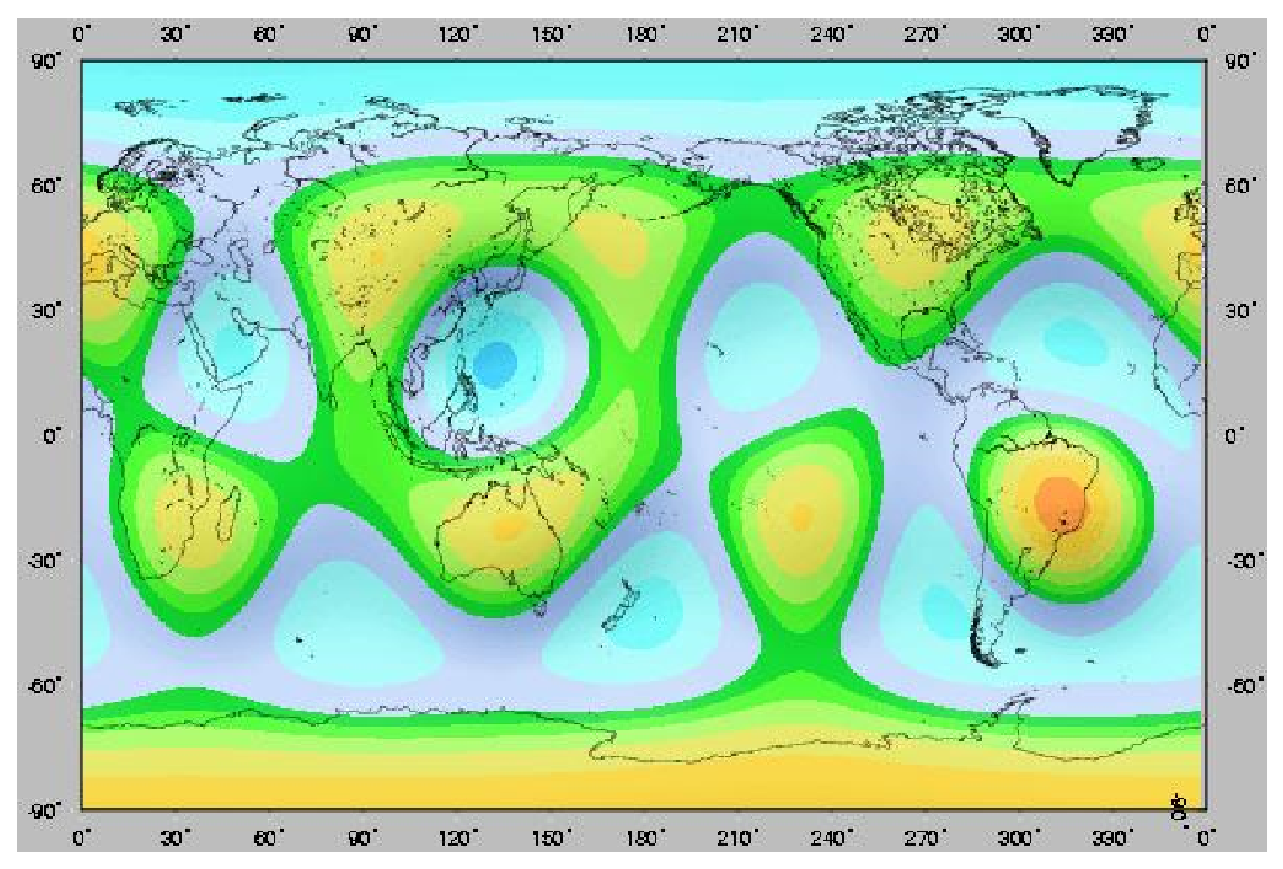
\includegraphics[width=0.3\textwidth]{earth_l5}} 
	\subfloat[$\ell=6$]{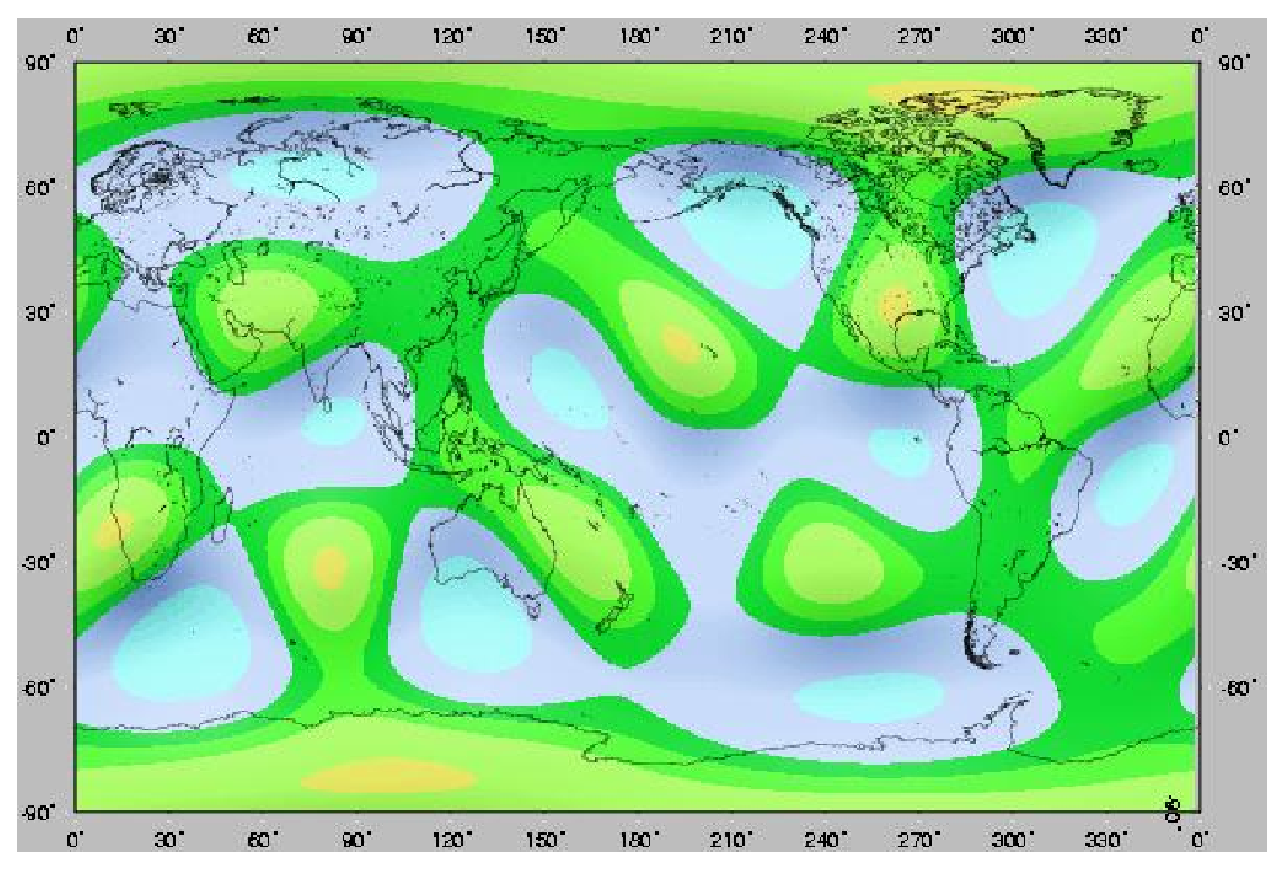
\includegraphics[width=0.3\textwidth]{earth_l6}}
	\caption{Spherical harmonics decomposition of earth topography. Source \ReferenceRef{Vigny}.}
	\label{fig:earth_decompo}
\end{figure}
\begin{figure}
	\ContinuedFloat
	\centering
	\subfloat[$\sum_{\ell=0}^6$]{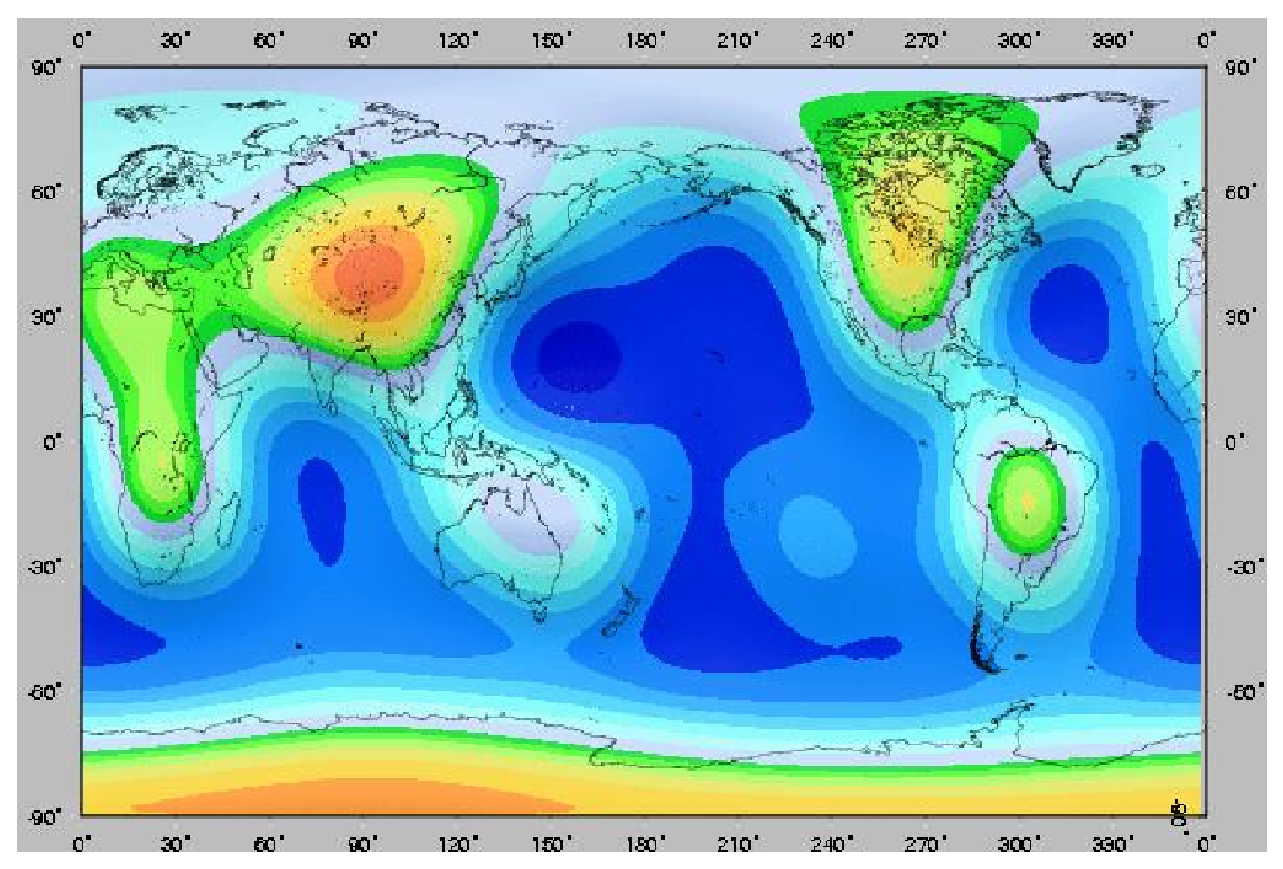
\includegraphics[width=0.45\textwidth]{earth_to6}} 
	\subfloat[$\sum_{\ell=0}^{16}$]{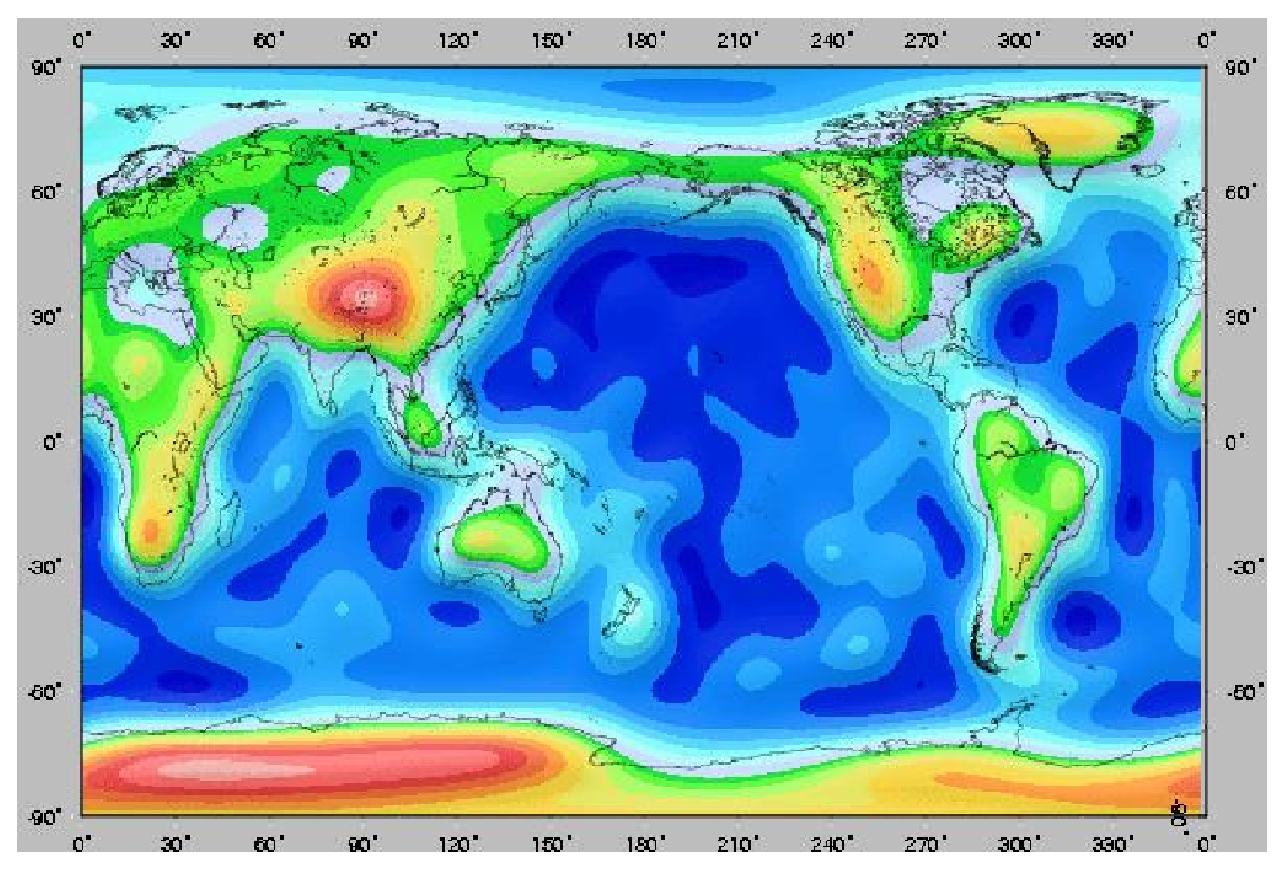
\includegraphics[width=0.45\textwidth]{earth_to16}}\\
	\subfloat[$\sum_{\ell=0}^{36}$]{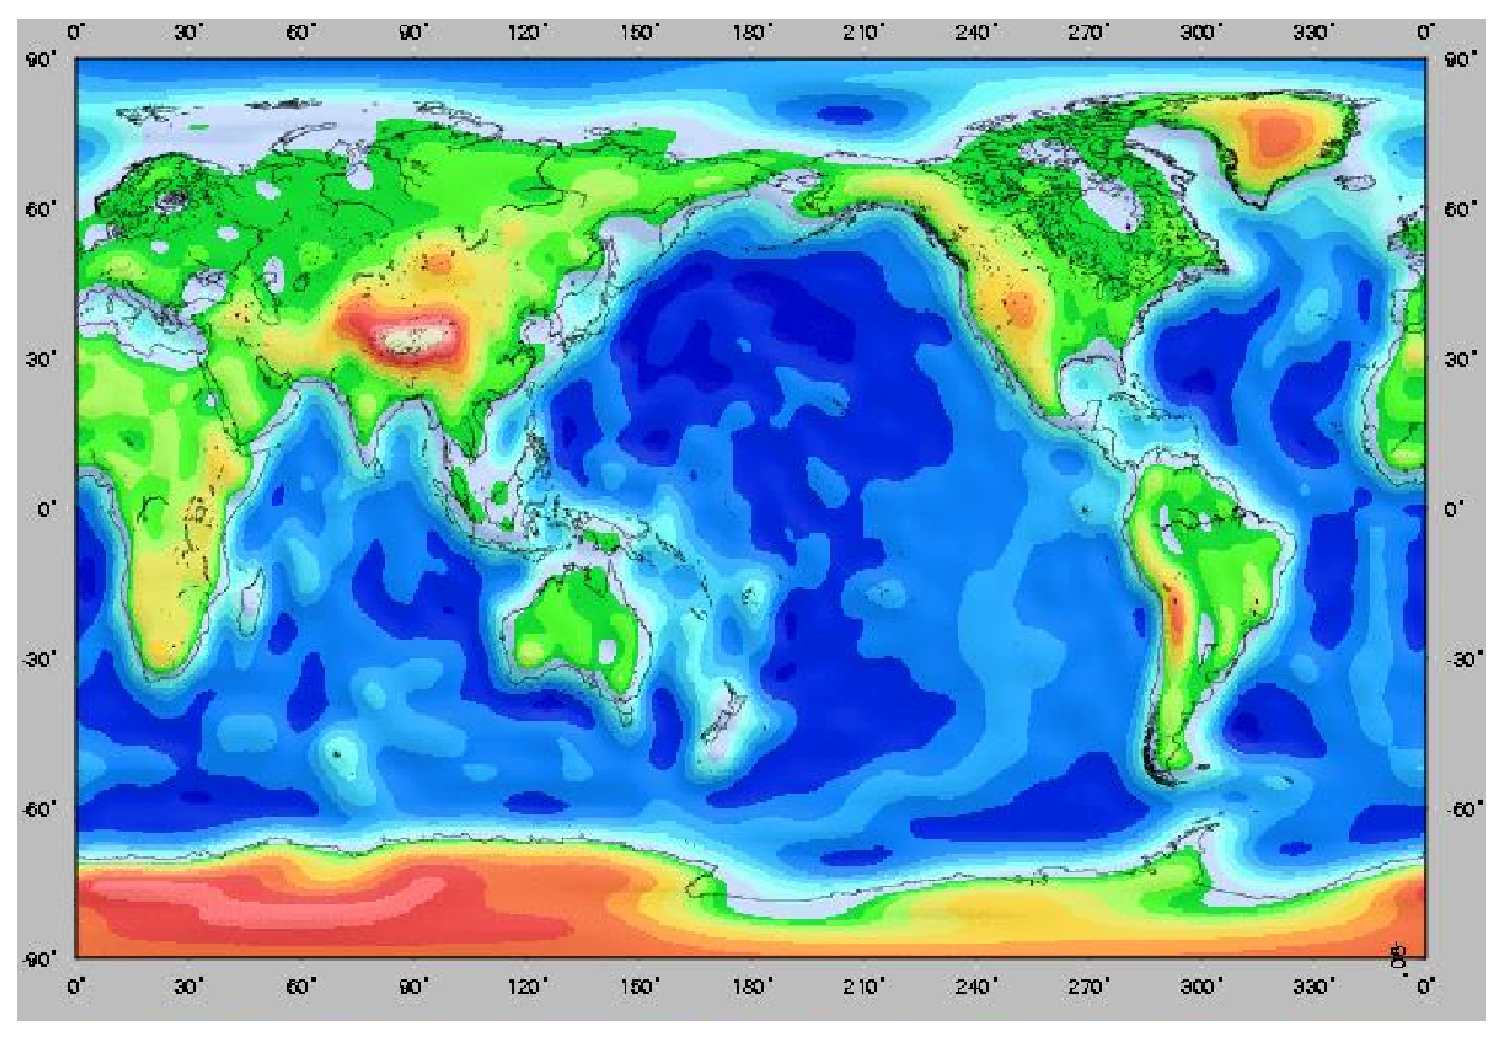
\includegraphics[width=0.45\textwidth]{earth_to36}} 
	\subfloat[Full grid of earth topography (6 data points per degree)]{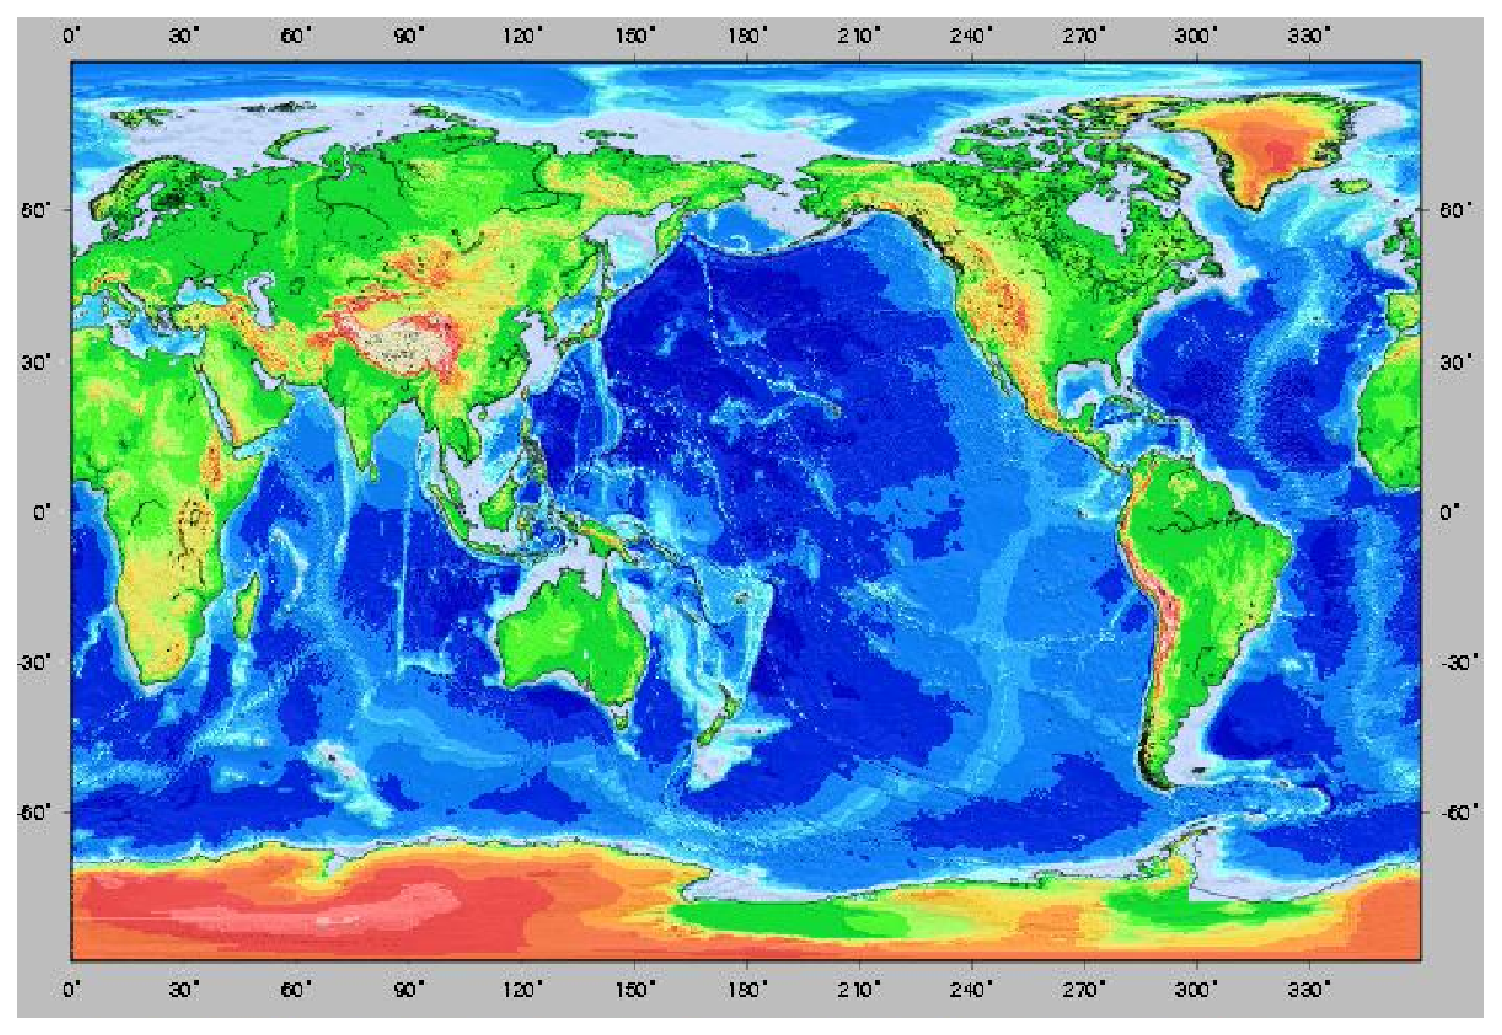
\includegraphics[width=0.45\textwidth]{earth_grid}}
	\caption{Approximations of earth topography by partial sums of spherical harmonics. Source \ReferenceRef{Vigny}.}
	\label{fig:earthApprox}
\end{figure}

\subsection{Characterisation of the bonds}

Each bond $\vec r$ can be associated with the set of spherical harmonics $Y_{\ell m}(\theta(\vec r),\phi(\vec r))$. For even $\ell$, there is no need to give a directionality to the bond. Often, the analysis is performed only on the $\ell=4$ and $\ell=6$ orders, the two first non-zero even orders in the spectrum (averaged over all bonds in the system). Some authors go up to $\ell=8$ and $\ell=10$~\citep{Chakravarty2002}.

The whole system is characterised by the coefficients $\bar{q}_{\ell m} = \langle Y_{\ell m}(\vec r) \rangle$ where the average is taken over all the bonds. Each particle $i$ is characterised by the coefficients
\begin{equation}
	q_{\ell m}(i) = \frac{1}{N_i}\sum_{0}^{N_i} Y_{\ell m}(\theta(\vec r_{ij}),\phi(\vec r_{ij}))
	\label{eq:qlm}
\end{equation}
where the $\vec{r}_{ij}$ are all the bonds starting from $i$. We call the $q_{\ell m}$ defined by \EquationRef{eq:qlm} the local tensorial bond orientational order parameter.

Other sums are possible, like adding the surface bonds into \EquationRef{eq:qlm}, \latin{i.e.} the bond $r_{jk}$ with $j$ and $k$ neighbours of $i$. The tensorial order parameter $q_{\ell m}$ can be calculated in this way for any subset of bonds. For example, any cluster found by a topological method can be considered as a set of bonds and thus have an associated $q_{\ell m}$.

\subsection{Invariants}
\label{sec:boo_invariants}
Because $q_{\ell m}$ can be scrambled drastically by a rotation of the coordinate system, it is important to consider combinations invariant by rotation like a normalised version of the spectrum coefficients:
\begin{align}
	q_\ell =& \sqrt{\frac{4\pi}{2l+1} \sum_{m=-\ell}^{\ell} |q_{\ell m}|^2 }\label{eq:ql}\\
	w_\ell =& \frac{
		\sum\limits_{m_1+m_2+m_3=0} 
			\left( \begin{array}{ccc}
				\ell & \ell & \ell \\
				m_1 & m_2 & m_3 
			\end{array} \right)
			q_{\ell m_1} q_{\ell m_2} q_{\ell m_3}
	}{
		\left(
			\sum\limits_{m=-\ell}^{\ell} |q_{\ell m}|^2
		\right)^{\frac{3}{2}}
	} \label{eq:wl}
\end{align}

The term in brackets is the Wigner 3-j symbol~\citep{Landau1965}. $q_\ell$ is always positive and indicates the strength of the $\ell$ fold symmetry. For instance, $q_6$ has high values for \ac{BCC}, \ac{HCP} and \ac{FCC} crystals as for icosahedron. $w_\ell$ can be positive or negative and gives more precise information about the symmetry group. For instance, Steinhardt \latin{et al.} showed that $w_6$ reaches its absolute minimum value only in the case of perfect icosahedral order:
\begin{equation}
w_6^{ico}= -\frac{11}{\sqrt{4199}} \sim -0.169
\label{eq:w6ico}
\end{equation}

Generally, the sign of $w_\ell$ indicates the parity of the $\ell$ fold symmetry. For example (see \FigureRef{fig:basicClusters}), \ac{HCP} and \ac{FCC} crystals have both high $q_6$ because they have both hexatic planes. But a \ac{HCP} crystal is made of the repetition of only two hexatic planes ($ABAB\ldots$), so its symmetry is even. Whereas a \ac{FCC} crystal is made of three planes ($ABCABC\ldots$) so its symmetry is odd. \ac{HCP}'s $w_4$ is positive and \ac{FCC}'s $w_4$ is negative. See \TableRef{tab:rotational_invarients} for the values of the rotational invariants for some basic structures.

\begin{table}
	\begin{center}
	\begin{tabular}{|l|r|r|r|r|r|r|r|r|}
		\hline
		Structure & $q_4$ & $q_6$ & $q_8$ & $q_{10}$ & $w_4$ & $w_6$ & $w_8$ & $w_{10}$ \\ \hline
		Ico. & 0 & 0.6633 & 0 & 0.3629 & $\infty$ & -0.1697 & $\infty$ & -0.0939 \\ \hline
		\ac{HCP} & 0.0972 & 0.4848 & 0.3170 & 0.0102 & 0.1341 & -0.0124 & 0.0513 & -0.0799 \\ \hline
		\ac{FCC} & 0.1909 & 0.5745 & 0.4039 & 0.0129 & -0.1593 & -0.0132 & 0.0584 & -0.0901 \\ \hline
		\ac{BCC} 9 & 0.5092 & 0.6285 & 0.2128 & 0.6502 & -0.1593 & 0.0132 & 0.0585 & -0.0901 \\ \hline
		\ac{BCC} 15 & 0.0364 & 0.5107 & 0.4293 & 0.1952 & 0.1593 & 0.0132 & 0.0585 & -0.0901 \\ \hline
		Dodec. & 0.0530 & 0.4298 & 0.1386 & 0.1401 & -0.1341 & -0.0937 & 0.0918 & 0.0077 \\ \hline
	\end{tabular}
	\end{center}
	\caption{Rotational invarients of a few perfect structures. $q_{\ell}$ are obtained from \EquationRef{eq:qlm} and \EquationRef{eq:ql}.}
	\label{tab:rotational_invarients}
\end{table}

In theory, every possible local structure could be identified using local bond orientational invariants. In practice, local bond order parameters are used in diverse ways. For instance, in \ReferenceRef{Desgranges2008}, the crystalline structure around a given particle is characterised by its position in the two dimensional $(q_4, q_6)$-plane and $(q_4, w_4)$-plane. Using this approach, one can determine the type of structure occurring around each individual particle. The values of the local invariants are in fact broadly distributed because of thermal fluctuations (see top of \FigureRef{fig:invariants_maps}). It is often not possible to tell if one given particle is in one structure or another.

Frenkel and co-workers~\citep{Moroni2005, wolde:9932, wolde1999homogeneous, Volkov2002} analysed the structure of crystalline clusters in terms of order parameter distributions. To do that, they first computed the distributions of $q_4$ and $q_6$ for the liquid and for perfect \ac{FCC} and \ac{BCC} crystals. Due to thermal fluctuations, these distributions can be rather broad (see \FigureRef{fig:invariantsFit}). Then, they determined the distributions of the same order parameters in the crystalline cluster. These distributions are represented as a superposition of the distribution functions of the perfect phases. The superposition coefficients $c_{FCC}$, $c_{BCC}$ and $c_{LIQ}$, determined by mean square minimisation, then yield information on the composition of the cluster. For instance, $c_{FCC} \approx 0.5$, $c_{BCC} \approx 0.5$, and $c_{LIQ} \approx 0$ would be indicative of a cluster that is half in the \ac{FCC} structure and half in the \ac{BCC} structure.

\begin{figure}
	\centering
	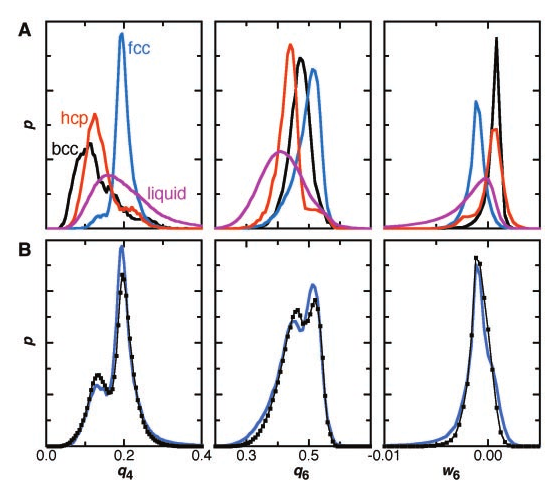
\includegraphics[width=0.8\textwidth]{gasser_invariants}
	\caption{(A) $q_4$, $q_6$, and $w_6$ bond-order parameter histograms for \acs{FCC} (blue curves), \acs{HCP} (red curves), \acs{BCC} (black curves), and liquid (purple curves). (B) The measured bond-order histograms (black plots) of a colloidal hard sphere sample with $\phi=0.45$ are shown together with a least squares fit (blue curve) using the bond-order histograms from (A). Source \ReferenceRef{Gasser2001}.}
	\label{fig:invariantsFit}
\end{figure}

\subsection{Correlations}
\label{sec:boo_correl}

Besides the rotational invariants, we can quantify the correlation between the $\ell$-fold symmetry around particle $i$ and particle $j$ by the following dot product:
\begin{equation}
	s_\ell(i,j) = \frac{
		\sum_{m=-\ell}^{\ell} q_{\ell m}(i) q_{\ell m}^{*}(j)
	}{
		\sqrt{\sum_{m=-\ell}^{\ell} |q_{\ell m}(i)|^2} \sqrt{\sum_{m=-\ell}^{\ell} |q_{\ell m}(j)|^2}
	}
	\label{eq:boo_dot_product}
\end{equation}

By definition $s_\ell(i,i)=1$. Note that this correlation depends on the relative orientation of the two environments: two exactly similar environments rotated one compared to the other by angles inconsistent with the $\ell$-fold symmetry would give low or even negative values of $s_\ell(i,j)$. Furthermore, $s_6(i,j)$ does not differentiate between two well oriented icosahedron and two well oriented \ac{FCC} neighbourhoods: both pairs would be strongly correlated.

The radial correlation function of the tensorial bond order can then be defined as:
\begin{equation}
	g_\ell(r) \equiv \frac{1}{N}\sum_i^N \frac{
		\sum_{j \neq i}{ s_\ell(i,j) \delta\left(\left\|\vec{r}_i-\vec{r}_j \right\| - r \right)}
	}{
	\sum_{j \neq i}{\delta\left(\left\|\vec{r}_i-\vec{r}_j \right\| - r \right)}
	}
	\label{eq:boo_space_correl}
\end{equation}

Tensorial correlations can also be defined in time in the spirit of \EquationRef{eq:boo_dot_product} by taking $i$ and $j$ at different times. Note that this tensorial time correlation is not robust to the global rotation of a cluster keeping the same structure.
\begin{equation}
	g_\ell(t) \equiv \left\langle \frac{
		\sum_{m=-\ell}^{\ell} q_{\ell m}(i, t_0) q_{\ell m}^{*}(i, t_0+t)
	}{
		\sqrt{\sum_{m=-\ell}^{\ell} \left\|q_{\ell m}(i,t_0)\right\|^2}
	}\right\rangle_{i, t_0}
	\label{eq:boo_time_correl}
\end{equation}


\subsection{Cluster detection}
\label{sec:X_bonds}

In order to study nucleation growth of crystals, one need to be able to know for sure if a particle is within a crystalline cluster or not. As we saw before, the local invariants $q_{\ell}(i)$ have broad distributions. Many insulated high $q_6$ particles are detected in a fluid. Frenkel \latin{et al.}~\citep{wolde:9932} had the idea to look at $s_6(i,j)$ when $i$ and $j$ are neighbouring particles. The bond $r_{ij}$ is considered a crystalline bond if $s_{ii}>0.5$. A particle is crystalline-like if its number of crystalline bonds is above a certain threshold, typically between 6 and 8. If a particle has less crystalline bonds, it is considered to be liquid-like. Using this criterion to distinguish crystalline-like from liquid-like particles one can then search for clusters of connected solid-like particles.

\begin{figure}
	\centering
	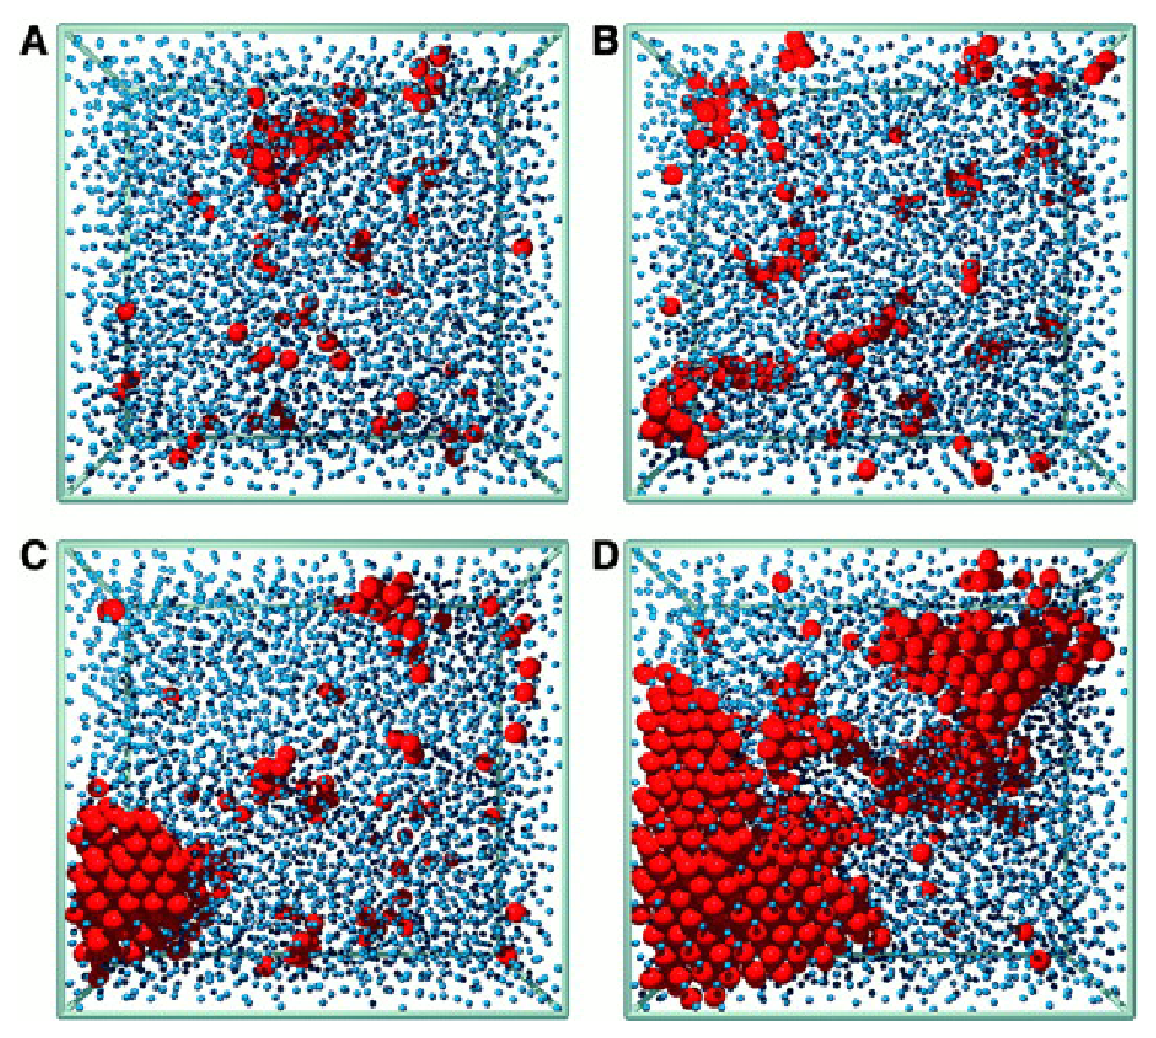
\includegraphics[width=0.8\textwidth]{gasser_nucleus}
	\caption{Four snapshots during crystallisation of a sample with $\phi=0.45$. The red spheres are drawn to scale and represent particles that were identified as crystal-like. The particles in the metastable liquid state are shown by the blue spheres, reduced in size for clarity. (A) Time $t=\unit{20}{\minute}$ after shear melting, (B) $t=\unit{43}{\minute}$, (C) $t=\unit{66}{\minute}$, and (D) $t=\unit{89}{\minute}$. Source \ReferenceRef{Gasser2001}}
	\label{fig:nucleus}
\end{figure}

This procedure very efficiently distinguishes between periodic environments and non-periodic environments, but does not discriminate between different crystal structures. Furthermore, it is not picking up the aperiodic structures like icosahedra. As noted by \citet{Tomida1995}, two adjacent icosahedra have different orientations, so $s_6(i,j)$ take negative values.

\subsection{Coarse graining}
\label{sec:cgBOO}

\begin{figure}
	\centering
	\subfloat[]{\label{fig:lech_q4q6}\def\svgwidth{0.45\textwidth}\input{lechner_q4q6.pdf_tex}}\quad
	\subfloat[]{\label{fig:lech_q4w4}\def\svgwidth{0.45\textwidth}\input{lechner_q4w4.pdf_tex}}\\
	\subfloat[]{\label{fig:lech_Q4Q6}\def\svgwidth{0.45\textwidth}\input{lechner_Q4Q6.pdf_tex}}\quad
	\subfloat[]{\label{fig:lech_Q4W4}\def\svgwidth{0.45\textwidth}\input{lechner_Q4W4.pdf_tex}}
	\caption{Top: Comparison between the $(q_4,q_6)$-plane \subref{fig:lech_q4q6} and the $(Q_4,Q_6)$-plane \subref{fig:lech_Q4Q6} for a Lennard-Jones system in three different crystalline structures and in the liquid phase. Each point corresponds to a particular particle, where \unit{2000}{points} from each structure were chosen randomly. Bottom: $(q_4,w_4)$-plane \subref{fig:lech_q4w4} and the $(Q_4,W_4)$-plane \subref{fig:lech_Q4W4}. Source \ReferenceRef{lechner:114707}.}
	\label{fig:invariants_maps}
\end{figure}

As mentioned above, thermal fluctuations smear out the order parameter distributions such that it may be difficult to distinguish local crystalline structures based on Steinhardt bond order parameters. \citet{lechner:114707} proposed to perform a coarse graining step, in order to take into account the second shell around each particle. They define the coarse-grained coefficients (that we note here with capital letters)
\begin{equation}
	Q_{\ell m}(i) = \frac{1}{\tilde{N} (i)} \sum_{k=0}^{\tilde{N}(i)} q_{\ell m}(k)
\end{equation}
Here, the sum from $k=0$ to $\tilde{N}(i)$ includes the neighbours of $i$ and $i$ itself. The coarse-grained invariants $Q_\ell$ and $W_\ell$ are derived from the $Q_{\ell m}$ the same way as \EquationRef{eq:ql} and \EquationRef{eq:wl}.

While $q_\ell(i)$ holds the information of the structure of the first shell around particle $i$, its averaged version $Q_\ell(i)$ also takes into account the second shell. One might say that using the parameter $Q_\ell$ instead of $q_\ell$ increases the accuracy of the distinction of different structures at the price of a coarsening of the spatial resolution.

As displayed in \FigureRef{fig:invariants_maps}, $Q_4$-$Q_6$-plane and $Q_4$-$W_4$-plane become very efficient maps to identify crystalline structures at a particle level. Because the overlap of bond orientational order distributions between crystalline structures become negligible, it is possible to categorise any given particle into a single structure. The distributions can be narrowed even further by averaging over a time characteristic to the vibrational motion~\citep{tanaka2010critical}.

As the crystalline bond method, the coarse-graining method relies on some amount of periodicity of the structures. The bond orientational order of the non-periodic structures gets averaged down by coarse-graining. This can be considered as a major drawback, or a mean to differentiate between periodic and aperiodic structures, as we will show in \ChapterRef{ch:structure}. For instance, the correlation function $G_\ell(i,j)$ of the coarse grained tensorial bond order (analogue to \EquationRef{eq:boo_space_correl}) only catches the fluctuations of the crystalline order, without interference of icosahedral order.

\subsection{Icosahedral order and mirror symmetry}
\label{sec:ico_mirror}

\begin{figure}
	\centering
	\subfloat[Sharing 7 particles: $\alpha$-interlocking]{\label{ico_19}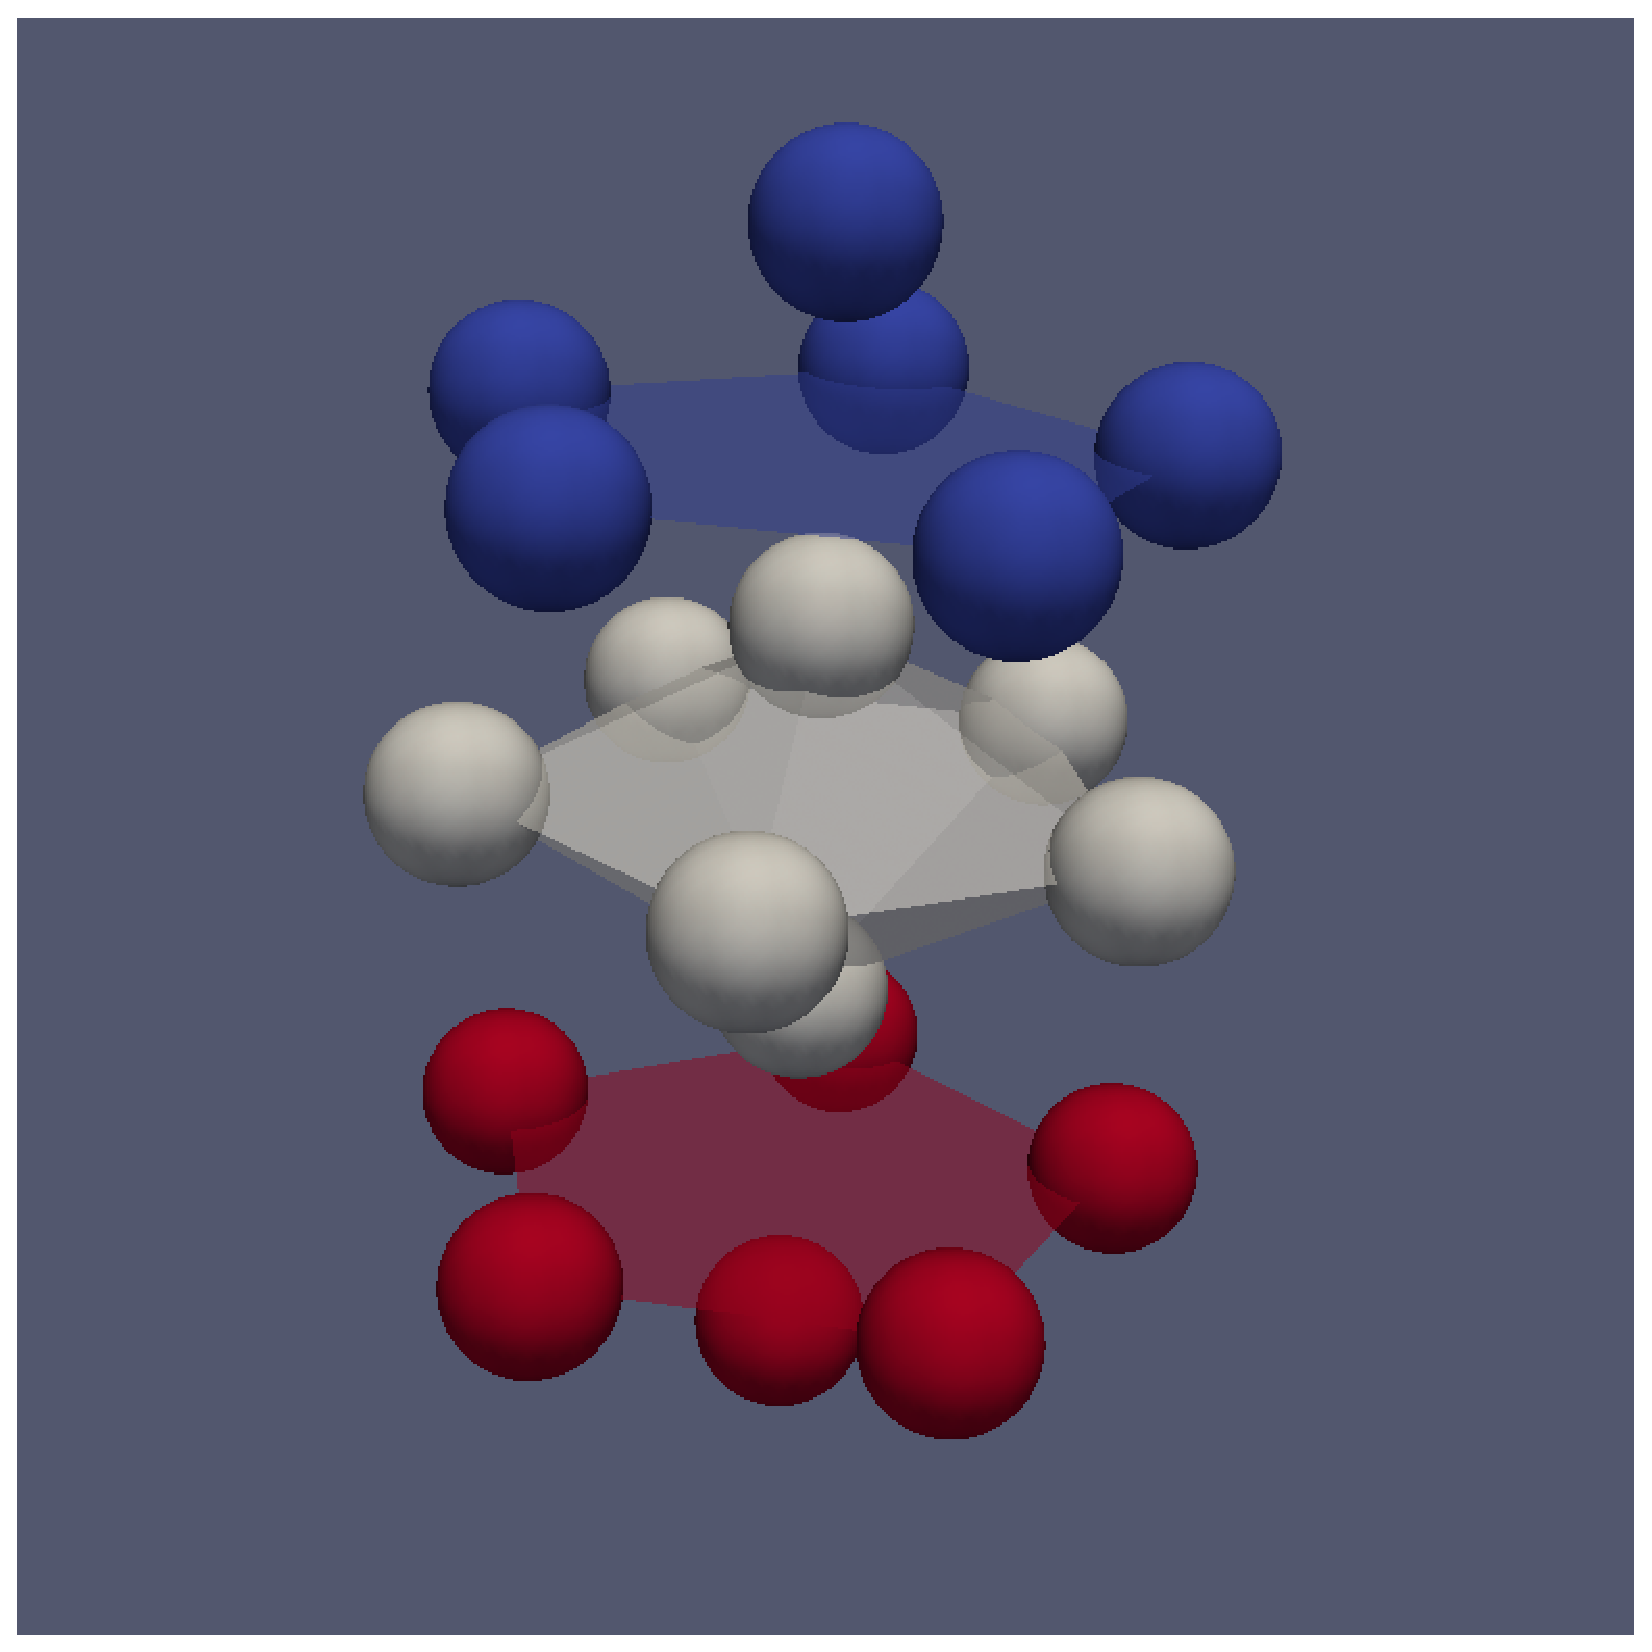
\includegraphics[width=0.3\textwidth]{ico_19}}\quad
	\subfloat[Sharing 3 particles: $\beta$-interlocking]{\label{ico_23}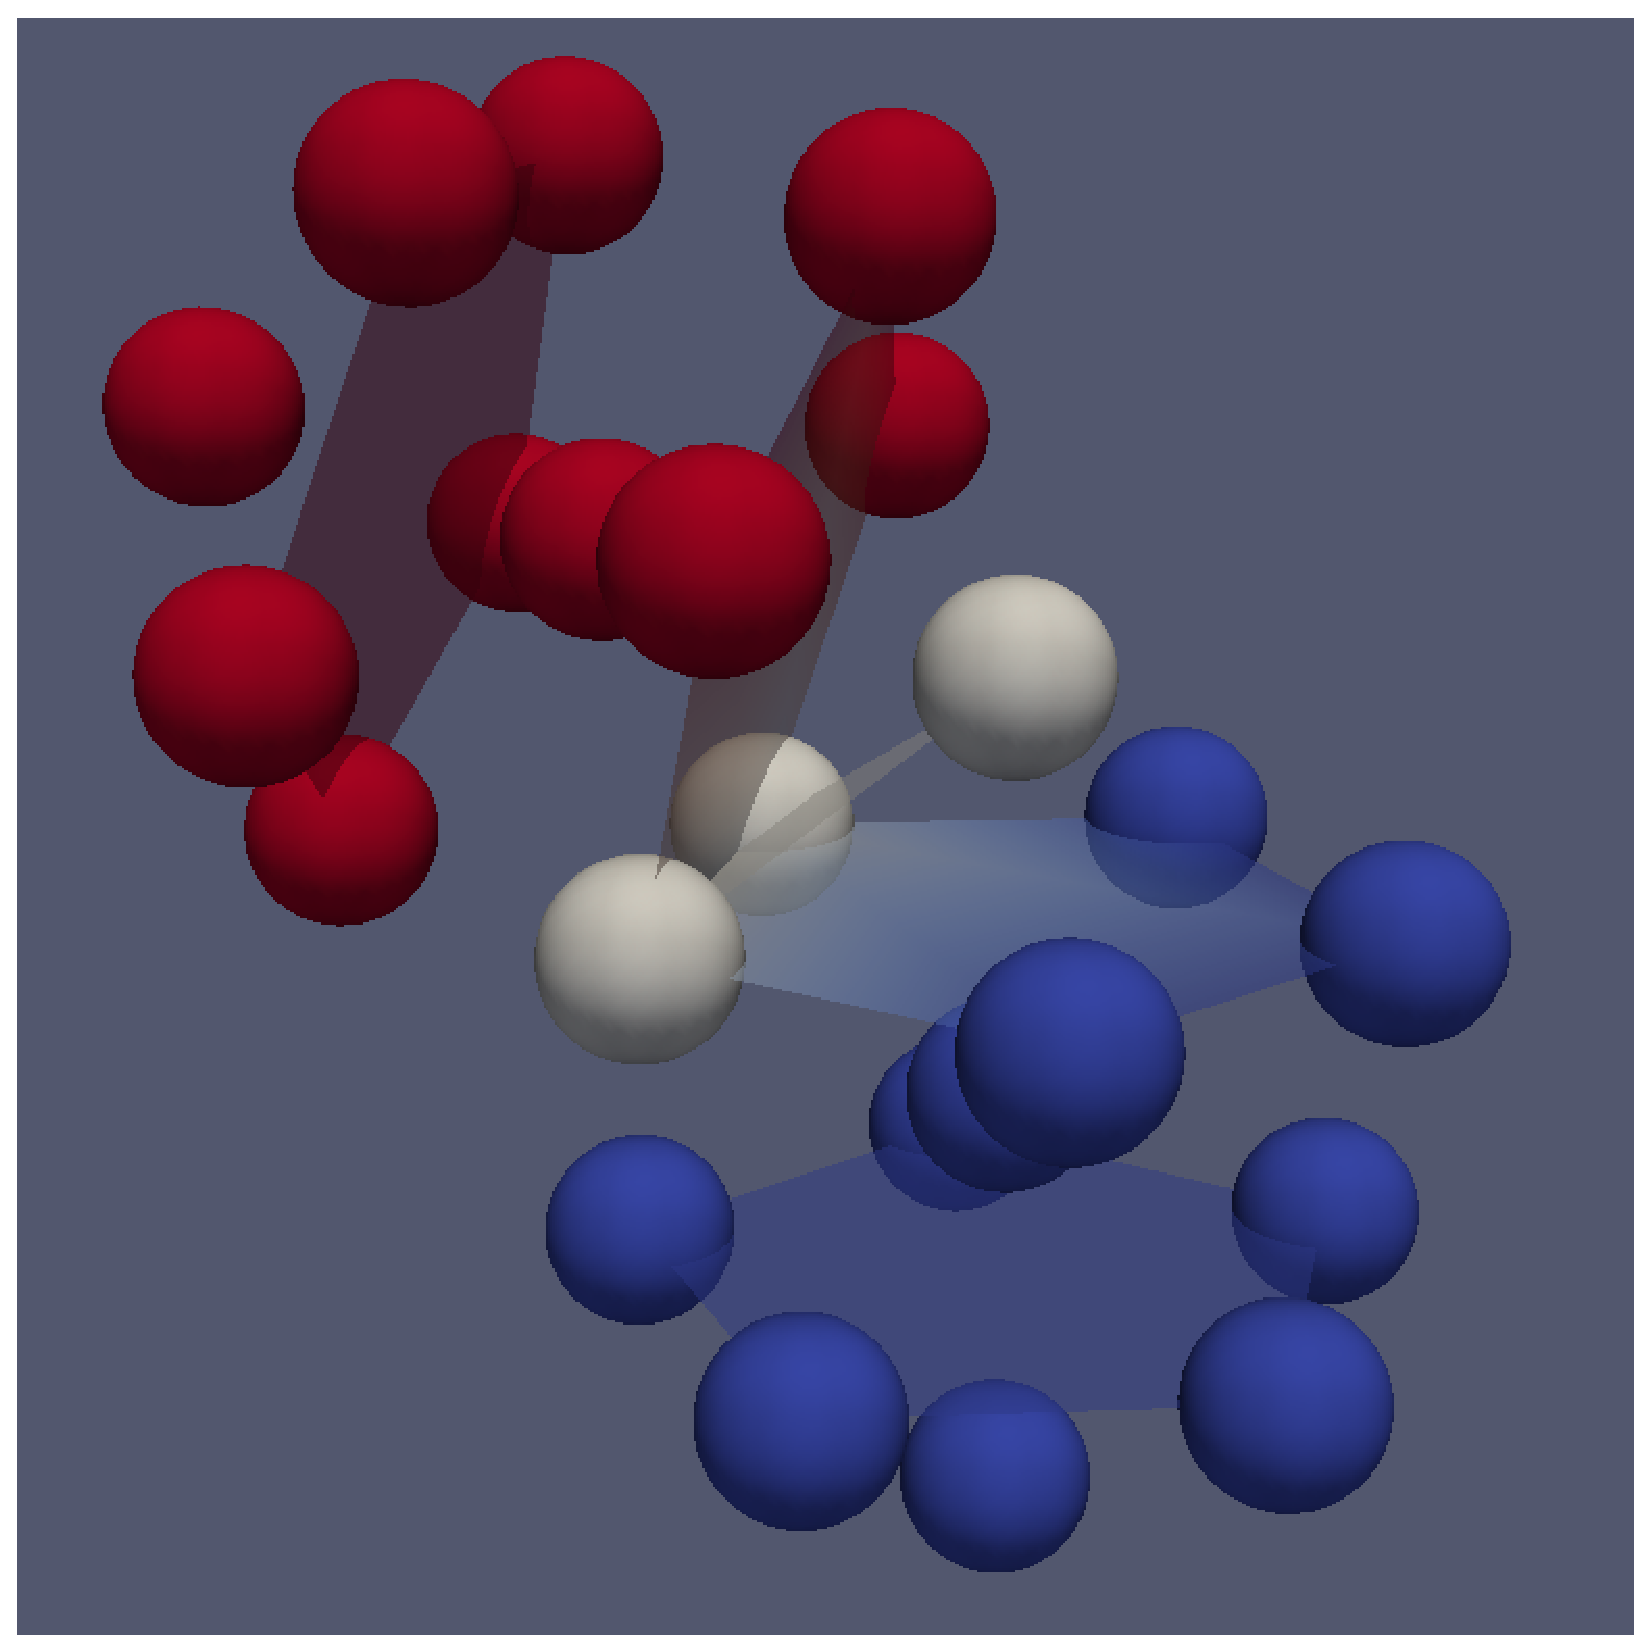
\includegraphics[width=0.3\textwidth]{ico_23}}
	\caption{Two simple interlocking states of icosahedral clusters. The blue icosahedron and the red one share the white particles. In both cases, the two icosahedra can be superimposed if mirrored by the plane defined by the common particles. In \subref{ico_19} the central particles of the icosahedra neighbours, whereas in \subref{ico_23} they are in each other's second shell.}
	\label{fig:ico_contact}
\end{figure}

Icosahedral order is a particular case in all the methods that involve the spatial extent of structures. This is because icosahedral order is not invariant by translation. \citet{Tomida1995} noticed that two icosahedra can share particles mainly in two ways depicted in \FigureRef{fig:ico_contact}: by sharing the 7 particles of a pentagonal di-pyramid ($\alpha$-interlocking) or by sharing the 3 particles of a face ($\beta$-interlocking). In the former, both icosahedra are elongated of about $10\%$ in the direction of their common axis. In both cases, the interlocking icosahedra cannot be superimposed by translation ($s_6(i,j)<0$), but they are related by mirror symmetry. 

\citet{Tomida1995} used this property to define a correlator that would indicate a perfect correlation between interlocked icosahedra. They define the operator $\mathcal{R}_{i j}$ as the reflection-symmetric operator against the median plane of the vector $\vec{r}_{i j}$. One can show that in the case of even $\ell$, the action of this operator on the spherical harmonics of degree $\ell$ is equivalent to a rotation of $\pi/2$ along $\vec{r}_{i j}$. The effect of $\mathcal{R}_{i j}$ on $q_{\ell m}$ can thus can be expressed by the rotation formula of spherical harmonics:
\begin{equation}
	\mathcal{R}_{i j}(q_{\ell m}) = \sum_{m'} D_{m, m'}^{(l)}\left(\alpha, \beta, \gamma \right) q_{\ell m'}
	\label{eq:rotate_boo}
\end{equation}
with $D_{m, m'}^{(l)}$ a Wigner D-matrix~\citep{Wigner1960} and $\alpha, \beta, \gamma$ the Euler angles of the rotation. The mirror-symmetry compatible correlation between neighbouring clusters $i$ and $j$ is then defined as:
\begin{equation}
	\kappa_\ell(i,j) \equiv \frac{
		\sum_{m=-\ell}^{\ell} q_{\ell m}(i) \mathcal{R}_{i j}\left(q_{\ell m}(j)\right)^{*}
	}{
		\sqrt{\sum_{m=-\ell}^{\ell} |q_{\ell m}(i)|^2} \sqrt{\sum_{m=-\ell}^{\ell} |q_{\ell m}(j)|^2}
	}
	\label{eq:boo_mirror_dot}
\end{equation}

We are tempted to define icosahedral bonds from $\kappa_\ell(i,j)$ as we defined crystalline bonds from $s_\ell(i,j)$ in \SectionRef{sec:X_bonds}. However, the mirror symmetry preserves the correlation between neighbouring crystalline environments. $\kappa_\ell(i,j)$ catches both crystalline and icosahedral bonds. \citet{Tomida1995} avoid this difficulty by defining their icosahedral bonds in a different way:
\begin{itemize}
	\item First they detect the icosahedra. The criterion is high $q_6$, that could in general catch also crystalline order, but the values of the other $q_\ell$ confirmed that the icosahedral order was the only one detectable in their system
	\item Second they detect the interlocking of the icosahedra by the topology of the bond network.
\end{itemize}

For icosahedra, the operator $\mathcal{R}_{i j}$ makes sense only between two interlocking clusters. If we imagine a chain of four interlocking icosahedra $1\rightarrow2\rightarrow3\rightarrow4$, the symmetry of the two terminal clusters are not directly related by the mirror symmetry $\mathcal{R}_{1 4}$. We have to flip three times along each interlocking state to recover the same orientation. The right operator is then $\mathcal{R}_{1 2}^{path} = \mathcal{R}_{1 2} \circ \mathcal{R}_{2 3} \circ \mathcal{R}_{3 4}$. In general, the correlation between icosahedra $i$ and $j$ has to be taken along the successive predefined icosahedra bonds, selecting the shortest path.


\section{Conclusion}

We reviewed a few methods to identify local structures in real space. For 2D isotropic interactions, $\psi_6$ is the reference method. TCC and coarse-grained bond orientational order are - at our knowledge - the state of the art. Topological approaches are better at detecting a great variety of structures, centred or not on a particle, periodic or not; but lack the ability to follow simple evolution or spatial extent of the structures. Bond orientational order approaches are very good at identifying crystalline order, even distorted or partial and its correlations in time or space. Icosahedral order is also accessible once the influence of eventual crystalline order has been removed.

We have not touched upon non-isotropic systems (non spherical shape, anisotropic potential) or multi-species systems. However, the local structure identification methods in these systems are - or will probably be - based on the simple isotropic one-specie scenario.

In the remaining chapters of this thesis, we will use the bond orientational order method, both coarse-grained and non coarse grained. Both the Voronoi and the maximum bond length methods were investigated to establish the bond network, however the bond orientational order computations based on the Voronoi bond network proved to be less consistent; thus all the results presented in the following chapters are based on the maximum bond length method.

%\newpage
% Create the bibliography right after the text
%\bibliographystyle{ieeetr}
%\bibliography{mathieu}

